\documentclass[aspectratio=169]{beamer}
\usetheme{Madrid}

\usepackage{lmodern}
\usepackage[utf8]{inputenc}
\usepackage[T1]{fontenc}
\usepackage[english]{babel}
\usepackage{amsmath,amssymb,bm}
\usepackage{graphicx}
\usepackage{booktabs}
\usepackage{multirow}
\usepackage{tikz}
\usetikzlibrary{decorations.pathreplacing}

% flat blocks: avoid Madrid shadow rendering artefacts
\setbeamertemplate{blocks}[rounded][shadow=false]

\graphicspath{{figures/}}

\title[HoTHP]{HoTHP: Hyperbolic Rotary Position Embedding-based Transformer Hawkes Process}
\subtitle{Length extrapolation in Temporal Point Processes}
\author[H. R. Soares]{Hugo Ramos Soares}
\institute[UFC]{Universidade Federal do Ceará \\[1em]
    {\small Orientador: César Lincoln C. Mattos (UFC)} \\
    {\small Coorientador: João Paulo Pordeus Gomes (UFC)} \\[0.3em]
    {\small Banca: José Antonio Fernandes de Macêdo (UFC) \\
    Diego Parente Paiva Mesquita (FGV)}
}
\date{Mestrado - Defesa Final, 28 de agosto de 2026}

\begin{document}

% ============================================================
% Slide 1: title
\begin{frame}
  \titlepage
\end{frame}

% ============================================================
% Opening hook (accessible framing before the technical content)
% ============================================================

% Hook slide 1: everything happens in time
\begin{frame}{Everything happens in time}
  \begin{columns}[T]
    \begin{column}{0.32\textwidth}
      \centering
      
\includegraphics[height=0.34\textheight,keepaspectratio]{hook_phone}\\[0.5em]
      {\small A message arrives.\\ Then another.}
    \end{column}
    \begin{column}{0.32\textwidth}
      \centering
      
\includegraphics[height=0.34\textheight,keepaspectratio]{hook_hospital}\\[0.5em]
      {\small A patient is seen,\\ and returns months later.}
    \end{column}
    \begin{column}{0.32\textwidth}
      \centering
      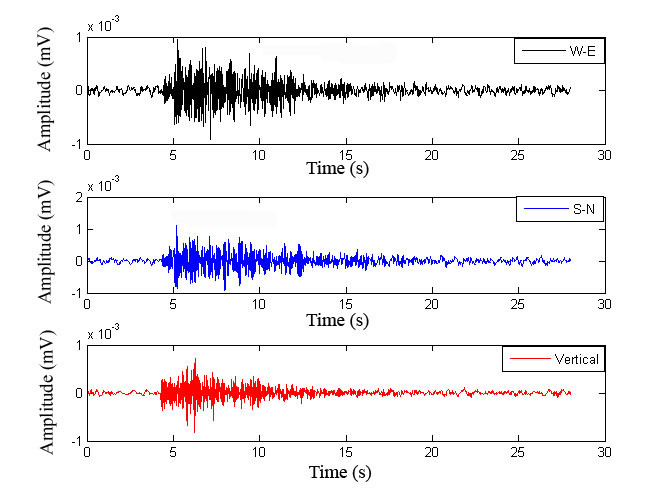
\includegraphics[height=0.34\textheight,keepaspectratio]{hook_seismogram}\\[0.5em]
      {\small The ground shakes.\\ When will it shake again?}
    \end{column}
  \end{columns}
  \vspace{0.8em}
  \begin{center}
    \large The question behind all of them:\\[0.25em]
    {\Large \textbf{when does the next one happen?}}
  \end{center}
  \vspace{0.3em}
  {\scriptsize\color{gray} Images: Wikimedia Commons.}
\end{frame}

% Hook slide 2: learn from little, predict far ahead
\begin{frame}{Learn from little, predict far ahead}
  \centering
  \vspace{0.6em}
  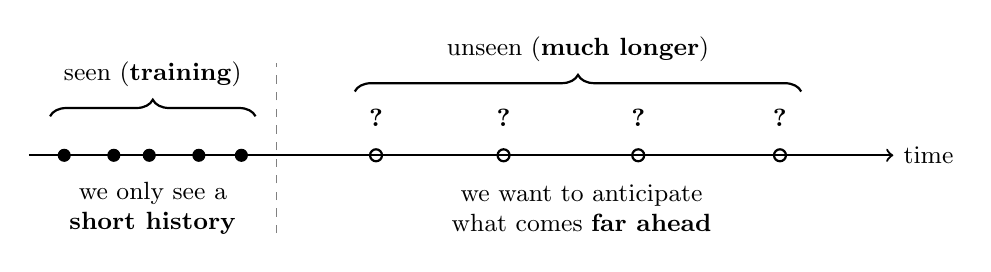
\begin{tikzpicture}[scale=0.9,every node/.style={font=\small}]
    % baseline
    \draw[->,thick] (0,0) -- (12.2,0) node[right]{time};
    % observed events (short history), close together
    \foreach \x in {0.5,1.2,1.7,2.4,3.0} \filldraw (\x,0) circle (2.4pt);
    % divider between seen and unseen
    \draw[dashed,gray] (3.5,-1.1) -- (3.5,1.3);
    % future events (sparse, unknown)
    \foreach \x in {4.9,6.7,8.6,10.6} {\draw[thick] (\x,0) circle (2.4pt);
      \node[above=3pt] at (\x,0.15) {\textbf{?}};}
    % braces
    \draw[decorate,decoration={brace,amplitude=6pt},thick] (0.3,0.55) -- (3.2,0.55)
      node[midway,above=7pt]{seen (\textbf{training})};
    \draw[decorate,decoration={brace,amplitude=6pt},thick] (4.6,0.9) -- (10.9,0.9)
      node[midway,above=7pt]{unseen (\textbf{much longer})};
    % bottom labels
    \node[align=center] at (1.75,-0.75) {we only see a\\ \textbf{short history}};
    \node[align=center] at (7.8,-0.75) {we want to anticipate\\ what comes \textbf{far ahead}};
  \end{tikzpicture}

  \vspace{1.0em}
  \begin{block}{The challenge of this work}
    \centering
    Train on \textbf{short} sequences of events, and stay reliable on
    \textbf{much longer} ones.
  \end{block}
\end{frame}

% Slide 2: outline
\begin{frame}{Outline}
  \tableofcontents
\end{frame}

% ============================================================
\section{Introduction}
% ============================================================

% Slide 3: real-world event sequences
\begin{frame}{Real-world event sequences}
  Many phenomena happen in continuous time and we need to model them:
  \vspace{0.4em}
  \begin{columns}[T]
    \begin{column}{0.25\textwidth}
      \centering
      \textbf{Telemetry} \\
      \small system failures, infrastructure alerts
    \end{column}
    \begin{column}{0.25\textwidth}
      \centering
      \textbf{Social networks} \\
      \small retweets, likes, reply cascades
    \end{column}
    \begin{column}{0.25\textwidth}
      \centering
      \textbf{Health} \\
      \small admissions, exams, prescriptions of a patient
    \end{column}
    \begin{column}{0.25\textwidth}
      \centering
      \textbf{Maintenance} \\
      \small failures in industrial equipment
    \end{column}
  \end{columns}
  \vspace{0.8em}
  \begin{block}{What do they have in common?}
    Each domain produces an ordered sequence of events with timestamps:
    \[
      \mathcal{S} = \{(t_1, k_1), (t_2, k_2), \ldots, (t_N, k_N)\}
    \]
    where $t_i$ is the time and $k_i$ is the type (mark) of event $i$.
  \end{block}
\end{frame}

% Slide 4: what we want to model
\begin{frame}{What do we want to model?}
  Given the past events, we want to answer:
  \begin{itemize}
    \item \textbf{When} will the next event happen?
    \item \textbf{Of which type} will it be?
  \end{itemize}
  \vspace{0.5em}
  The central tool is the \textbf{conditional intensity}:
  \[
    \lambda(t \mid \mathcal{H}_t) = \lim_{\Delta t \to 0}
      \frac{P(\text{event in } [t, t+\Delta t) \mid \mathcal{H}_t)}{\Delta t}
  \]
  where $\mathcal{H}_t$ is the history of all events before $t$.
  \vspace{0.5em}
  \begin{block}{Learning objective}
    Learn $\lambda(t)$ from data so that the model generalizes to sequences
    with lengths different from those seen during training.
  \end{block}
\end{frame}

% Slide 5: the practical problem + contribution
\begin{frame}{The practical problem: train short, test long}
  \begin{itemize}
    \item Collecting long event sequences is often expensive or impractical.
    \item We would like to \textbf{train on short sequences} and run the model on
          \textbf{arbitrarily longer} ones \cite{press2022train}.
    \item Transformer-based point process models degrade sharply when the test
          sequence is longer than the training one. The ability to remain stable
          in this regime is called \emph{length extrapolation}.
  \end{itemize}
  \vspace{0.6em}
  \begin{block}{Contribution of this work: HoTHP}
    A Transformer Hawkes Process whose attention kernel is \textbf{hyperbolic}
    instead of trigonometric. It embeds an \textbf{exponential recency bias}
    directly in the attention, mirroring the structure of the Hawkes process, and
    keeps the likelihood stable under length extrapolation.
  \end{block}
\end{frame}

% Slide: objective and research question
\begin{frame}{Objective and research question}
  \begin{block}{Research question}
    Does replacing the \textbf{oscillatory} kernel with a kernel that has
    \textbf{exponential decay} in the attention mechanism improve the length
    extrapolation ability of neural temporal point processes?
  \end{block}
  \vspace{0.5em}
  To answer it, we:
  \begin{itemize}
    \item propose and implement the \textbf{HoTHP}, adapting HoPE from discrete
          positions to continuous time instants;
    \item evaluate it under \emph{train short, test long} on \textbf{synthetic}
          data (known generating process) and \textbf{real} data from varied
          domains;
    \item analyze \emph{under which conditions} the recency bias is beneficial,
          neutral, or harmful (learned intensities, accuracy, RMSE, and a
          temporal-scale ablation).
  \end{itemize}
\end{frame}

% ============================================================
\section{Foundations: Temporal Point Processes}
% ============================================================

% Slide 6: Poisson distribution (NEW)
\begin{frame}{The Poisson distribution}
  \textbf{The question it answers:} how many events will we see in a fixed
  window, if they happen independently at a constant average rate?
  \vspace{0.3em}
  \begin{block}{Definition \cite{ross_first_2019}}
    If the \emph{expected number} of events in the window is $\lambda > 0$, the
    probability of observing exactly $k$ events is
    \[
      \Pr(X = k) = \frac{\lambda^{k} e^{-\lambda}}{k!}, \qquad k = 0, 1, 2, \ldots
    \]
    \vspace{-0.6em}
    {\footnotesize
    \begin{itemize}
      \item $X$: a \textbf{random variable}, the count of events in the window
            (unknown before we observe it);
      \item $k$: a \textbf{concrete value} that count may take ($0, 1, 2, \ldots$);
      \item $\Pr(X = k)$: the \textbf{probability} that the observed count $X$
            equals exactly $k$.
    \end{itemize}}
  \end{block}
  {\small
  \begin{itemize}
    \item $\lambda$ is both the \textbf{mean} and the \textbf{variance} of the count.
  \end{itemize}}
\end{frame}

% Slide 7: Poisson process
\begin{frame}{The Poisson process}
  Now let events keep happening over time, at a constant \textbf{rate}
  $\lambda$ (events per unit time), and let $N(T)$ count them up to time $T$
  \cite{ross_first_2019}. Roughly:
  \begin{itemize}
    \item events in short, \textbf{non-overlapping} intervals happen
          \textbf{independently};
    \item each short interval gets \textbf{at most one} event, with chance
          proportional to $\lambda$.
  \end{itemize}
  Then $N(T)$ is Poisson with mean $\lambda T$ (rate times time):
  \[
    \Pr\{N(T) = n\} = \frac{(\lambda T)^{n}}{n!}\, e^{-\lambda T}
  \]
  \vspace{-0.3em}
  \begin{center}
    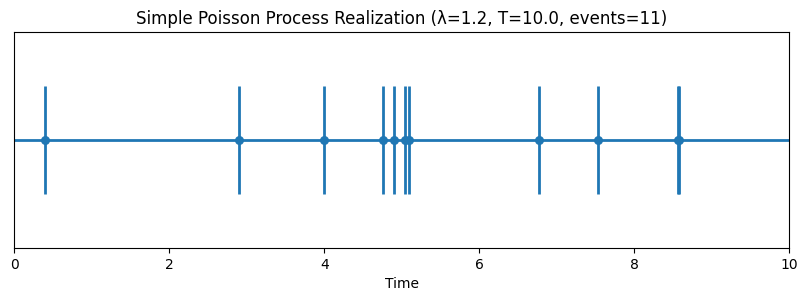
\includegraphics[width=0.56\textwidth]{figura-poisson}
  \end{center}
\end{frame}

% Slide 8: Temporal Point Processes
\begin{frame}{Temporal Point Processes (TPP)}
  Probabilistic models for sequences of discrete events in \textbf{continuous
  time} \cite{zuo2020transformer}. They handle events at irregular, arbitrary
  times.
  \vspace{0.3em}
  \begin{itemize}
    \item Fully described by the conditional intensity $\lambda(t \mid \mathcal{H}_t)$.
    \item With \textbf{marks} (event types), the sequence is
          $X = \{(t_1, m_1), \ldots, (t_N, m_N)\}$ and we use $K$ intensities:
  \end{itemize}
  \[
    \lambda_k(t \mid \mathcal{H}_t) = \lim_{\Delta t \to 0}
    \frac{\Pr(\text{event of type } k \text{ in } [t, t+\Delta t) \mid \mathcal{H}_t)}{\Delta t}
  \]
  \begin{block}{Note on the word ``mark''}
    We use \emph{mark} and \emph{type} interchangeably: the mark is a categorical
    event type, one of $K$ classes.
  \end{block}
\end{frame}

% Slide 9: Loss function (NEW own slide)
\begin{frame}{Loss function: the log-likelihood}
  Given all events observed in $[0,T]$, TPPs are trained by maximizing the
  log-likelihood \cite{mei2017neural}:
  \[
    \mathcal{L} = \sum_{i:\, t_i \leq T} \log \lambda_{k_i}(t_i)
      \;-\; \underbrace{\int_{0}^{T} \bar{\lambda}(t)\, dt}_{\Lambda},
    \qquad \bar{\lambda}(t) = \sum_{k=1}^{K} \lambda_k(t)
  \]
  \begin{itemize}
    \item First term: rewards a \textbf{high intensity} at the moments where
          events actually occurred (and for the right type $k_i$).
    \item Second term (the \emph{compensator} $\Lambda$): penalizes intensity mass
          where no event occurred.
    \item Training minimizes the \textbf{negative} log-likelihood (NLL), our main
          evaluation metric.
  \end{itemize}
  In practice, the integral is estimated numerically, in exactly the same way for
  every model we compare.
\end{frame}

% Slide 10: Hawkes process
\begin{frame}{The Hawkes process}
  Poisson assumes independent events. The \textbf{Hawkes process} assumes that
  \textbf{past events raise the probability of future events}, with an influence
  that decays exponentially \cite{hawkes1971spectra}:
  \[
    \lambda(t \mid \mathcal{H}_t) = \mu + \sum_{t_i < t} \alpha \, e^{-\beta (t - t_i)}
  \]
  \begin{columns}[T]
    \begin{column}{0.52\textwidth}
      \begin{itemize}
        \item $\mu$: baseline intensity.
        \item $\alpha$: instantaneous jump caused by an event.
        \item $\beta$: how fast that influence decays.
      \end{itemize}
      \vspace{0.3em}
      The exponential decay is a \textbf{recency bias}: recent events matter more.
    \end{column}
    \begin{column}{0.46\textwidth}
      \centering
      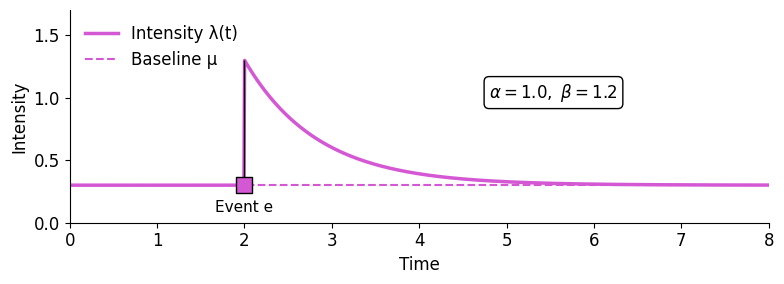
\includegraphics[width=\textwidth]{figura-hawkes}
    \end{column}
  \end{columns}
\end{frame}

% Slide 11: Cox process (NEW)
\begin{frame}{The Cox process, and where Hawkes sits}
  Increasingly rich ways of specifying the intensity:
  \vspace{0.4em}
  \begin{enumerate}
    \item \textbf{Homogeneous Poisson:} intensity $\lambda$ is constant.
    \item \textbf{Non-homogeneous Poisson:} $\lambda(t)$ varies in time, but
          deterministically.
    \item \textbf{Cox process} (doubly stochastic Poisson): $\lambda(t)$ is itself
          a \emph{random} process, driven by factors external to the events.
    \item \textbf{Hawkes process:} $\lambda(t)$ is random
          because it depends on the \emph{past events of the process itself}, each
          one temporarily raising the intensity.
  \end{enumerate}
  \vspace{0.5em}
  \begin{block}{Why this matters here}
    Hawkes also has a stochastic intensity, but unlike Cox its randomness is
    \textbf{endogenous}: $\lambda(t)$ is a functional of the process's own past (a
    \emph{self-exciting} process, not a doubly stochastic one). It is exactly this
    dependence on history, with exponential decay, that motivates the recency bias
    of our model.
  \end{block}
\end{frame}

% ============================================================
\section{Neural models and attention}
% ============================================================

% Slide 12: Neural Hawkes Process
\begin{frame}{Neural Hawkes Process (NHP)}
  The classical Hawkes process is limited: influence is always excitatory,
  constant per type, and decays exponentially. Mei and Eisner \cite{mei2017neural} relax
  these assumptions with neural networks.
  \begin{itemize}
    \item Allow $\alpha, \mu \in \mathbb{R}$, so events can \textbf{inhibit} as
          well as excite; a \textbf{softplus} keeps the intensity positive.
    \item Replace the additive sum by a \textbf{continuous-time LSTM} (CT-LSTM):
          the memory cell decays exponentially between events.
  \end{itemize}
  \[
    \lambda_k(t) = f_k\!\left(\mathbf{w}_k^\top \mathbf{h}(t)\right), \qquad
    \mathbf{c}(t) = \bar{\mathbf{c}} + (\mathbf{c} - \bar{\mathbf{c}})\,
      e^{-\bm{\delta}(t - t_i)}
  \]
  A simple but strong model: still a top benchmark today, and an important
  baseline in our experiments.
\end{frame}

% Slide 13: Transformers and attention
\begin{frame}{Transformers and the attention mechanism}
  RNNs (including the CT-LSTM) process events \textbf{sequentially}, which is slow
  and struggles with long sequences. The Transformer \cite{vaswani2017attention}
  removes recurrence: all events are processed at once through \textbf{attention}.
  \[
    \text{Attention}(Q,K,V) = \text{softmax}\!\left(\frac{QK^\top}{\sqrt{d_k}}\right) V
  \]
  \begin{itemize}
    \item Each event attends to every other event; the weights measure relevance.
    \item \textbf{Multi-head} attention runs $h$ projections in parallel and
          concatenates them.
  \end{itemize}
  \vspace{-0.2em}
  \begin{figure}
    \centering
    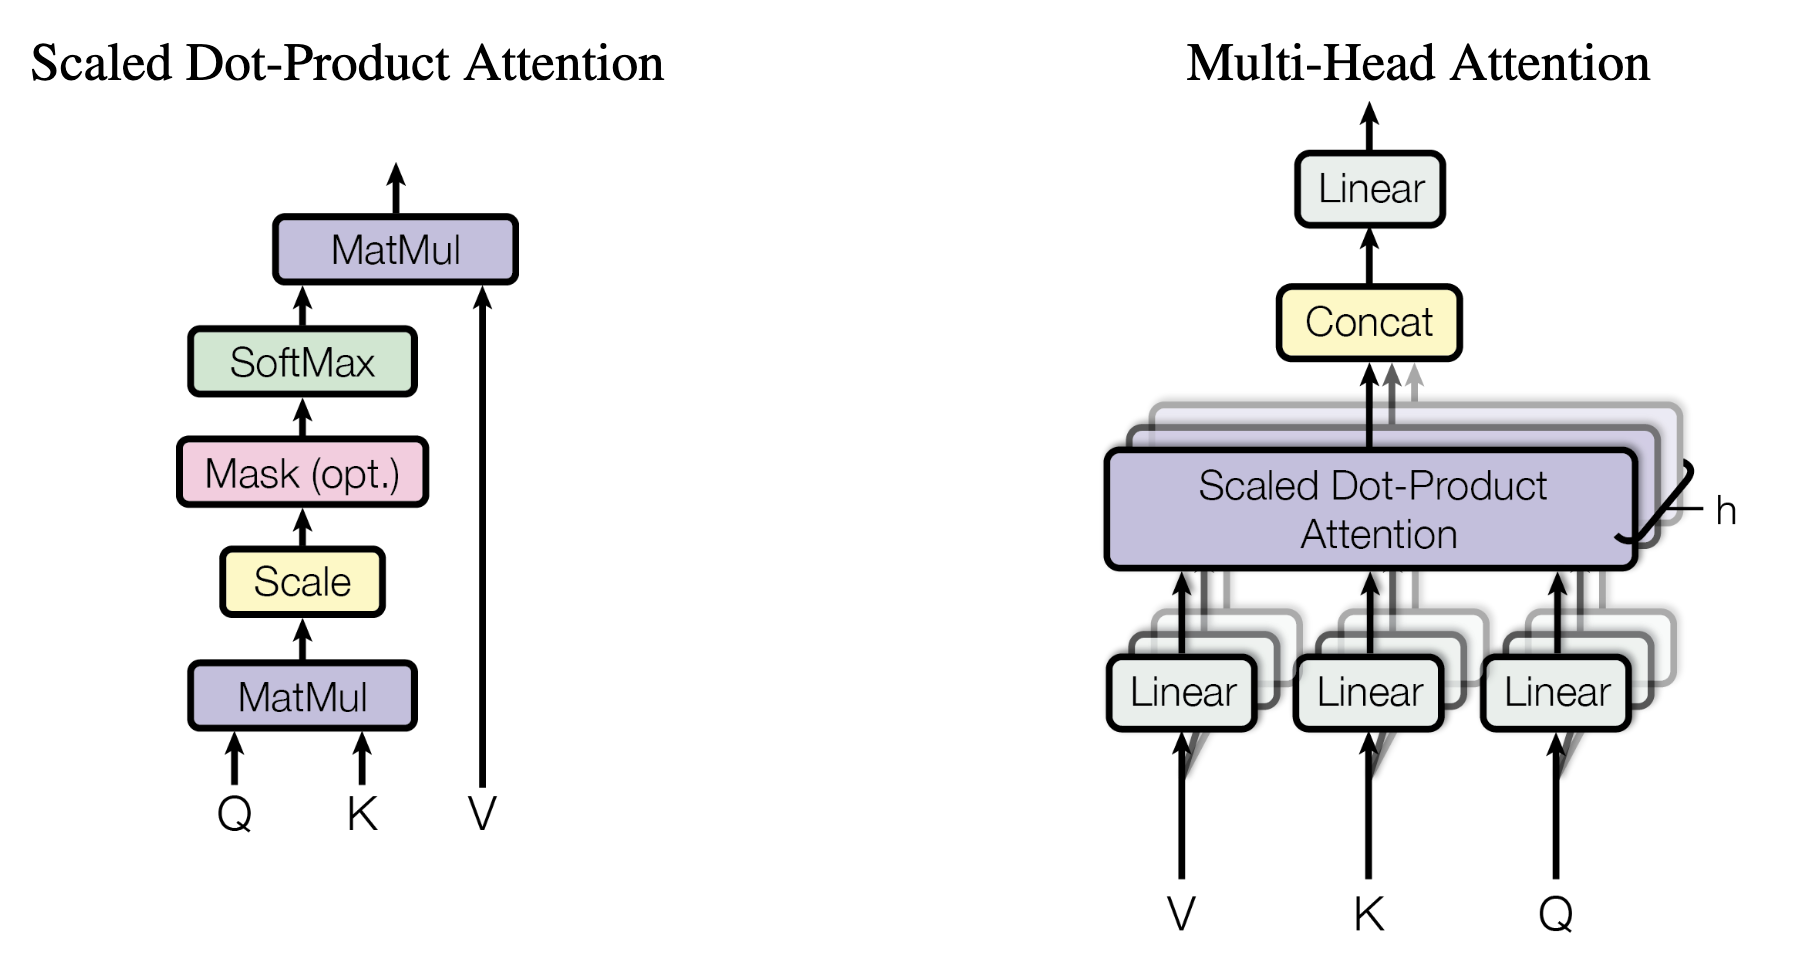
\includegraphics[height=0.32\textheight,keepaspectratio]{figura-attention}

    {\tiny\color{gray} Source: \cite{vaswani2017attention}}
  \end{figure}
\end{frame}

% Slide 14: positional encoding
\begin{frame}{Positional encoding: attention has no order}
  Attention is \textbf{permutation equivariant}: reordering the inputs merely
  reorders the outputs, so on its own it does not know the order or timing of
  events. Position must be injected.
  \vspace{0.3em}
  \begin{columns}[T]
    \begin{column}{0.54\textwidth}
      \small
      \begin{itemize}
        \item \textbf{Original Transformer:} add a sinusoidal encoding of the
              \emph{discrete position} to each token embedding.
        \item Each dimension is a sine/cosine of a different frequency: fast on
              the left, slow on the right, giving every position a unique
              signature.
        \item \textbf{For TPPs} we need the actual \emph{timestamp}, not just the
              order, since the moment of the event matters.
      \end{itemize}
    \end{column}
    \begin{column}{0.44\textwidth}
      \centering
      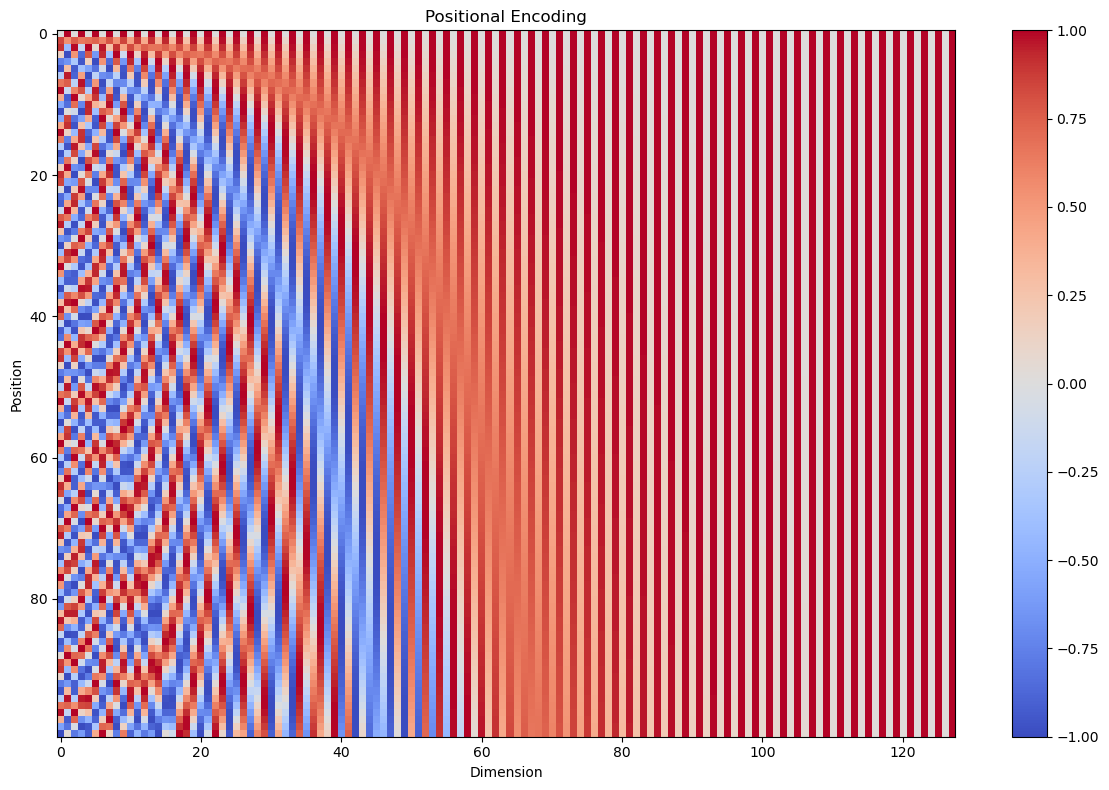
\includegraphics[width=\textwidth,height=0.62\textheight,keepaspectratio]{fig_positional_encoding}

      {\scriptsize Sinusoidal encoding: position (rows) vs. dimension (columns).}
    \end{column}
  \end{columns}
\end{frame}

% Slide 15: THP
\begin{frame}{Transformer Hawkes Process (THP)}
  Zuo et al. \cite{zuo2020transformer} adapt the Transformer to TPPs with a
  \textbf{temporal encoding} that uses the timestamp $t_j$ instead of a discrete
  position:
  \[
    [z(t_j)]_i =
    \begin{cases}
      \cos\!\left(t_j / 10000^{(i-1)/M}\right), & i \text{ odd},\\[2pt]
      \sin\!\left(t_j / 10000^{i/M}\right), & i \text{ even}.
    \end{cases}
  \]
  \vspace{-0.8em}
  \begin{columns}[T]
    \begin{column}{0.54\textwidth}
      The encoding is added to the type embedding, then passed through
      self-attention and a feed-forward network. The intensity is
      \[
        \resizebox{\linewidth}{!}{$
        \lambda_k(t) = f_k\!\Big(
          \underbrace{\alpha_k \tfrac{t-t_j}{t_j}}_{\text{current}}
          + \underbrace{\mathbf{w}_k^\top \mathbf{h}(t_j)}_{\text{history}}
          + \underbrace{b_k}_{\text{base}}\Big)
        $.}
      \]
    \end{column}
    \begin{column}{0.44\textwidth}
      \centering
      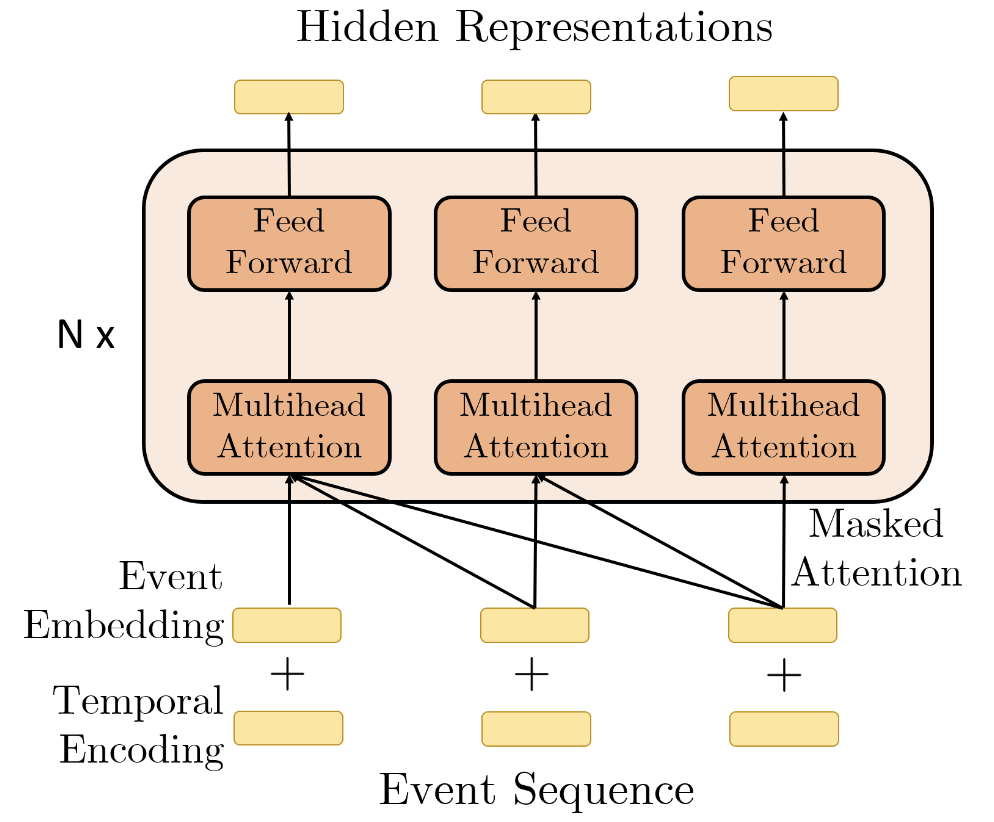
\includegraphics[width=0.80\textwidth,height=0.47\textheight,keepaspectratio]{figura-thp}\\[0.2em]
      {\tiny\color{gray} Source: \cite{zuo2020transformer}}
    \end{column}
  \end{columns}
\end{frame}

% ============================================================
\section{Related work: length extrapolation}
% ============================================================

% Slide 16: extrapolation in LLMs
\begin{frame}{Length extrapolation in language models}
  A model trained on sequences of length $L_{\text{train}}$ should stay stable when
  tested on $L_{\text{test}} > L_{\text{train}}$ \cite{press2022train}.
  \vspace{0.3em}
  \begin{columns}[T]
    \begin{column}{0.52\textwidth}
      \begin{itemize}
        \item Absolute sinusoidal positions produce encoding patterns never seen in training for larger indices: perplexity explodes.
        \item Rotary encodings (RoPE) help by using \emph{relative} positions, but
              Press et al. \cite{press2022train} showed they still fail for much
              longer sequences.
        \item Only \textbf{ALiBi}, with a linear distance penalty, stays flat far
              beyond the training length.
      \end{itemize}
    \end{column}
    \begin{column}{0.46\textwidth}
      \centering
      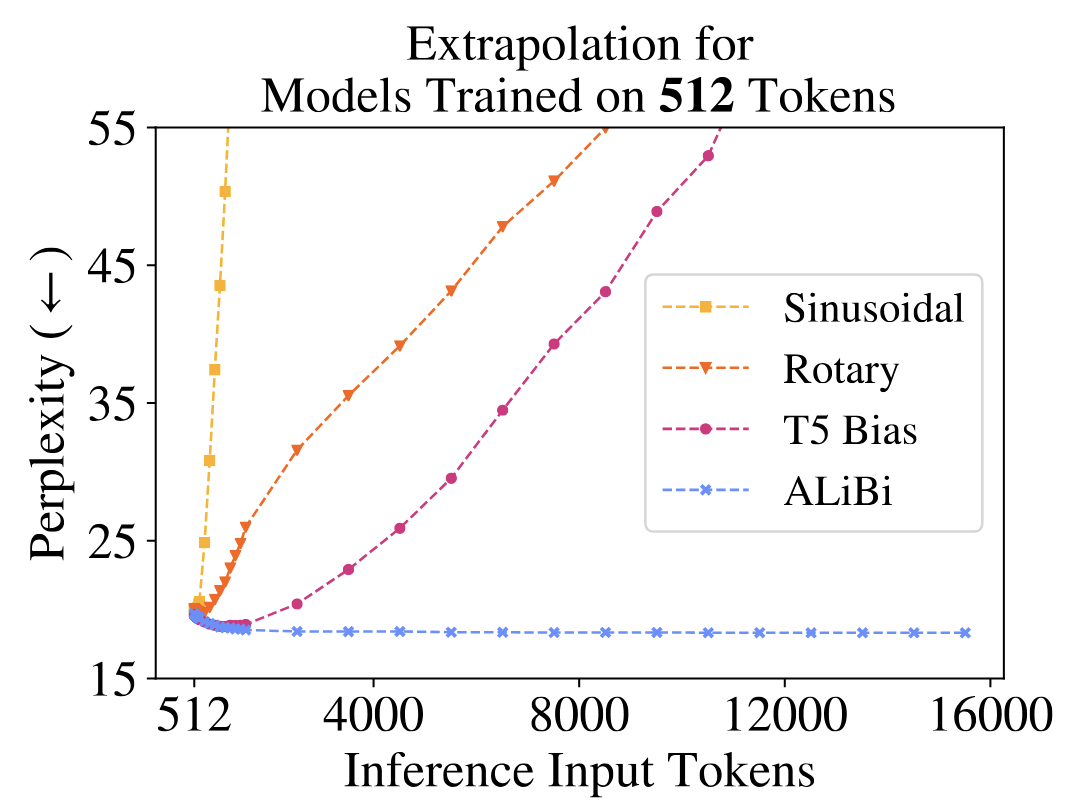
\includegraphics[width=\textwidth,height=0.56\textheight,keepaspectratio]{fig_alibi_extrapolation}\\[0.2em]
      {\tiny\color{gray} Source: \cite{press2022train}}
    \end{column}
  \end{columns}
\end{frame}

% Slide 17: same problem in TPPs
\begin{frame}{The same problem in TPPs: train short, test long}
  We adapt the \emph{train short, test long} protocol \cite{press2022train} to
  point processes, using the \textbf{number of events} as the length.
  \vspace{0.4em}
  \begin{itemize}
    \item Train on sequences of a fixed length (e.g. $L = 50$ events).
    \item Test on sequences $\alpha$ times longer, $\alpha \in \{1, 2, 5, 10\}$.
    \item At $\alpha = 10\times$: train on 50 events, test on 500.
  \end{itemize}
  \vspace{0.5em}
  \begin{block}{What we measure}
    Whether the NLL stays stable as $\alpha$ grows. A model with a proper recency
    bias should barely degrade.
  \end{block}
\end{frame}

% Slide 18: RoPE
\begin{frame}{Rotary Position Embedding (RoPE)}
  Su et al. \cite{su2024roformer} noticed that attention only needs the
  \textbf{relative} position. RoPE rotates pairs of embedding dimensions by an
  angle proportional to the position:
  \[
    \mathbf{R}_j(\Delta) =
    \begin{bmatrix} \cos(\theta_j \Delta) & \sin(\theta_j \Delta) \\
                   -\sin(\theta_j \Delta) & \cos(\theta_j \Delta) \end{bmatrix},
    \qquad \theta_j = 10000^{-2(j-1)/d}.
  \]
  \begin{columns}[T]
    \begin{column}{0.5\textwidth}
      \begin{itemize}
        \item Applied to $\mathbf{q}$ and $\mathbf{k}$ before the dot product.
        \item The score ends up depending only on the difference of positions.
      \end{itemize}
    \end{column}
    \begin{column}{0.5\textwidth}
      \centering
      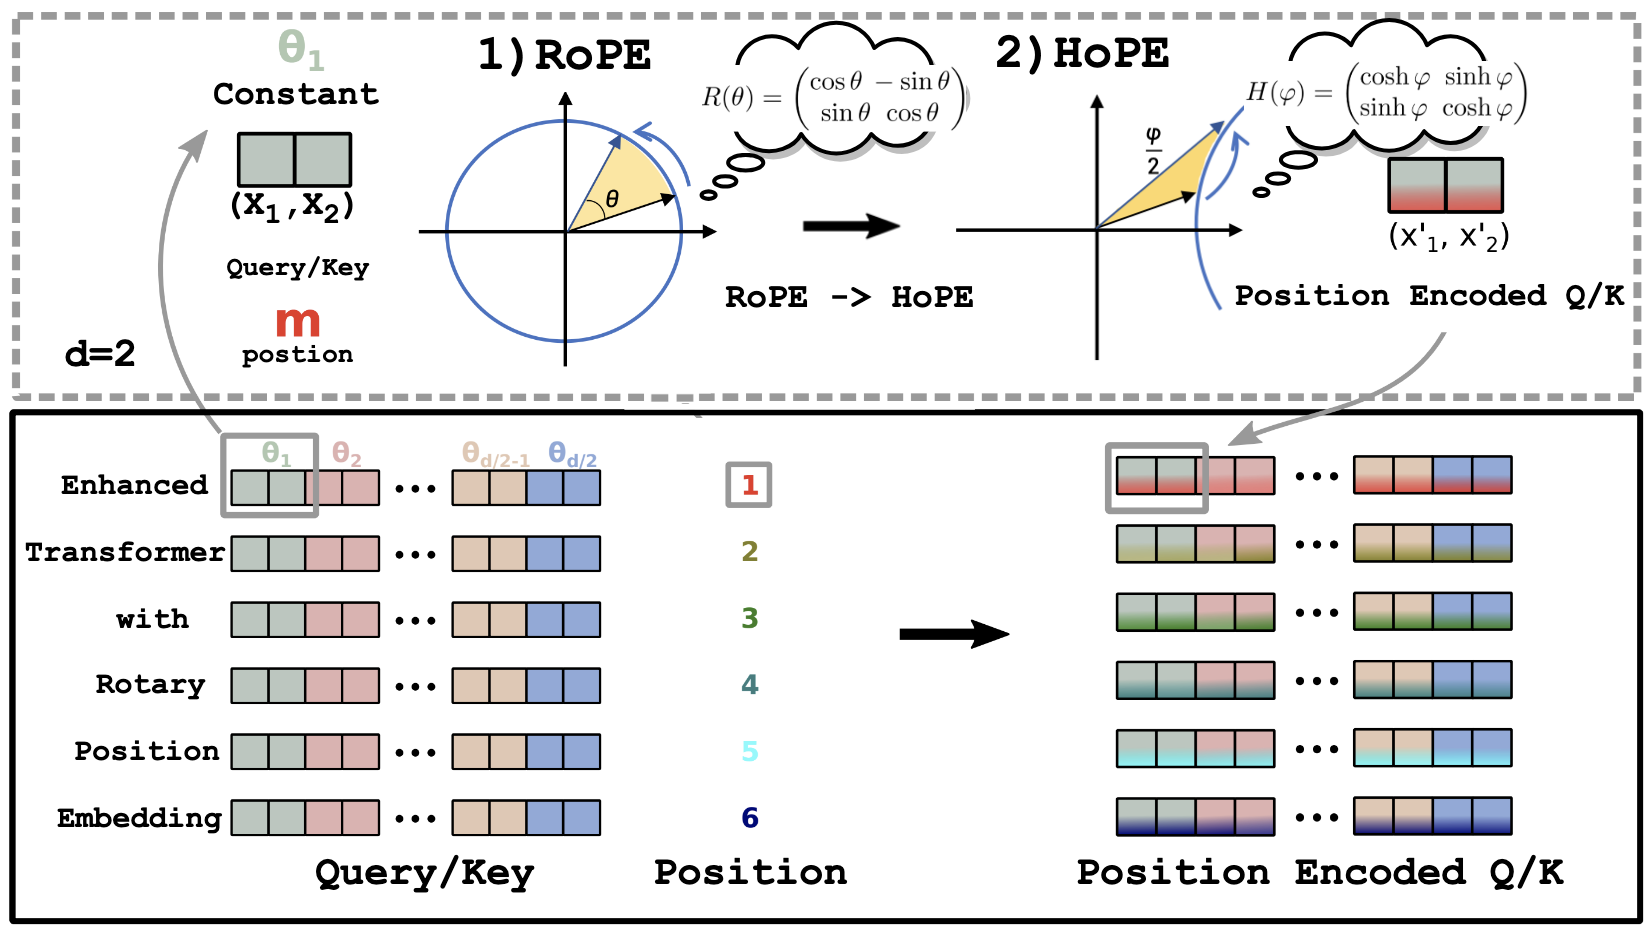
\includegraphics[width=0.85\textwidth,height=0.53\textheight,keepaspectratio]{fig_rope_to_hope}\\[0.2em]
      {\tiny\color{gray} Adapted from \cite{su2024roformer}}
    \end{column}
  \end{columns}
\end{frame}

% Slide 19: RoTHP
\begin{frame}{RoTHP: RoPE for point processes}
  Dai et al. \cite{dai2026rothp} bring RoPE to TPPs: rotate by the \textbf{timestamp}
  instead of the discrete index.
  \vspace{0.4em}
  \begin{itemize}
    \item The attention score depends only on $\Delta t = t_i - t_j$.
    \item This makes the likelihood \textbf{time-invariant}: shifting all times by
          a constant $\sigma$ leaves the result unchanged.
    \item Robust to timestamp noise (clock desynchronization), common in real
          data. New state of the art on several TPP benchmarks.
  \end{itemize}
  \vspace{0.4em}
  \begin{block}{But there is a catch}
    The rotary kernel is built from $\cos$ and $\sin$: it \textbf{oscillates}. This
    is the limitation our method addresses.
  \end{block}
\end{frame}

% Slide 20: ALiBi + recency bias (NEW)
\begin{frame}{ALiBi and the recency inductive bias}
  Press et al. \cite{press2022train} take a different route: no embedding at all, just a
  fixed \textbf{linear penalty} on the attention score:
  \[
    \text{softmax}\!\left(\mathbf{q}_i \mathbf{K}^\top
      + m \cdot [-(i{-}1), \ldots, -2, -1, 0]\right)
  \]
  \begin{itemize}
    \item The penalty grows with distance, so distant tokens are suppressed. The
          slope $m$ is fixed per head, never learned.
    \item This is an \textbf{inductive bias toward recency}, built into the
          architecture rather than learned from data.
  \end{itemize}
  \begin{block}{The connection to Hawkes}
    This is exactly the Hawkes kernel idea (influence $\propto e^{-\beta \Delta t}$
    decays with distance). THP and RoTHP dropped this structural guarantee when
    they replaced the kernel with free attention. \textbf{HoTHP puts it back.}
  \end{block}
\end{frame}

% ============================================================
\section{Methodology: HoTHP}
% ============================================================

% Slide 21: RoTHP oscillation limitation
\begin{frame}{The oscillatory limitation of RoTHP}
  RoTHP's score depends only on $\Delta t = t_i - t_j$, but its kernel is built
  from $\cos$ and $\sin$, so it \textbf{oscillates} instead of decaying.
  \begin{columns}[T]
    \begin{column}{0.44\textwidth}
      \begin{itemize}
        \item \textbf{RoPE} (blue) decays only \emph{on average}: noisy,
              non-monotonic, and it never dies out.
        \item A Hawkes kernel $\varphi(\Delta t)=\alpha e^{-\beta\Delta t}$ is
              \emph{strictly} decreasing. RoPE violates this.
        \item In extrapolation the phase may land on a \textbf{peak}: a distant
              event outscores a nearby one.
      \end{itemize}
      \vspace{0.2em}

    \end{column}
    \begin{column}{0.56\textwidth}
      \centering
      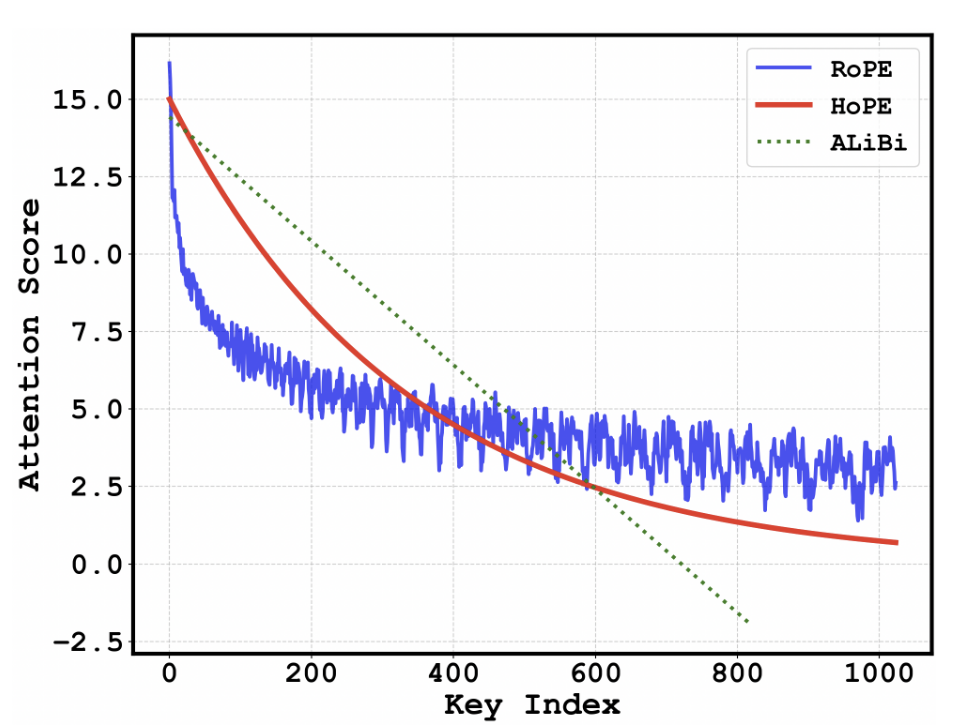
\includegraphics[width=\textwidth,height=0.72\textheight,keepaspectratio]{figura-oscilacao}
    \end{column}
  \end{columns}
\end{frame}

% Slide 22: trig -> hyperbolic
\begin{frame}{From the trigonometric kernel to the hyperbolic kernel}
  Following HoPE \cite{dai2025hope}, replace the rotation block $\mathbf{R}_j$ by a
  \textbf{hyperbolic boost} $\mathbf{B}_j$:
  \[
    \resizebox{0.78\textwidth}{!}{$
    \mathbf{R}_j(\Delta t) =
      \begin{bmatrix} \cos & \sin \\ -\sin & \cos \end{bmatrix}
    \;\longrightarrow\;
    \mathbf{B}_j(\Delta t) =
      \begin{bmatrix} \cosh(\theta_j \Delta t) & \sinh(\theta_j \Delta t) \\
                      \sinh(\theta_j \Delta t) & \cosh(\theta_j \Delta t) \end{bmatrix}
    $}
  \]
  \vspace{-0.4em}
  \begin{center}
    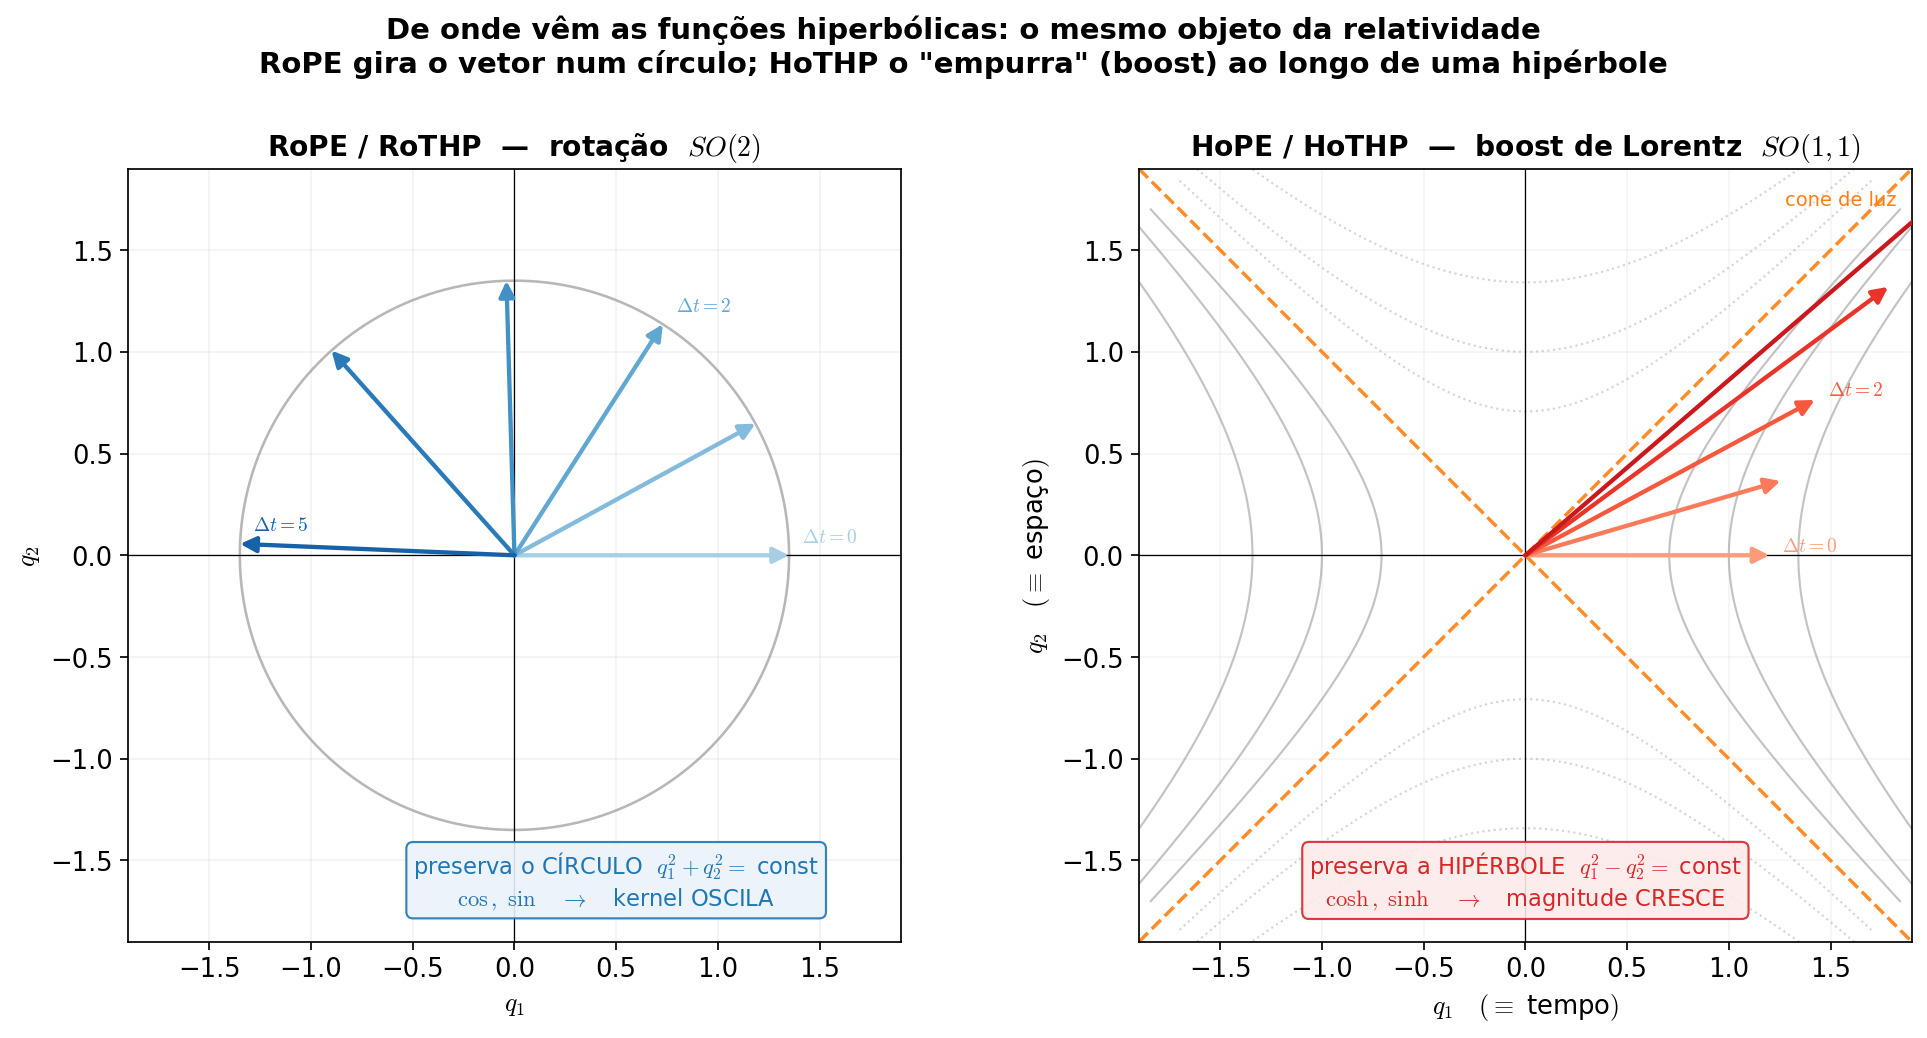
\includegraphics[width=0.92\textwidth,height=0.5\textheight,keepaspectratio]{fig_rope_vs_hothp_geom}
  \end{center}
  \vspace{-0.4em}
  {\footnotesize The rotation preserves the \textbf{circle} ($\cos,\sin$ oscillate); the
  Lorentz boost preserves the \textbf{hyperbola} ($\cosh,\sinh$ are monotonic). We control this growth  with the decay envelope
  $e^{-|\Delta t|\theta'}$.}
\end{frame}

% Slide 23: exponential decay + theta prime
\begin{frame}{Exponential decay and the parameter $\theta'$}
  HoPE \cite{dai2025hope} adds a learnable $\theta'$ and damps $\mathbf{q}, \mathbf{k}$
  so the score decays. In continuous time:
  \[
    g(\Delta t) = e^{-|\Delta t|\,\theta'}\; \mathbf{q}^\top \mathbf{B}(\theta, \Delta t)\, \mathbf{k}
  \]
  \begin{columns}[T]
    \begin{column}{0.5\textwidth}
      \begin{itemize}
        \item If $\theta' > \max_j \theta_j$, the decay dominates the hyperbolic
              growth: the score \textbf{decays exponentially to zero} with
              $|\Delta t|$, without oscillation.
        \item This is a \textbf{structural} recency bias: it holds even for
              $\Delta t$ never seen in training. This is what enables
              extrapolation.
      \end{itemize}
    \end{column}
    \begin{column}{0.5\textwidth}
      \centering
      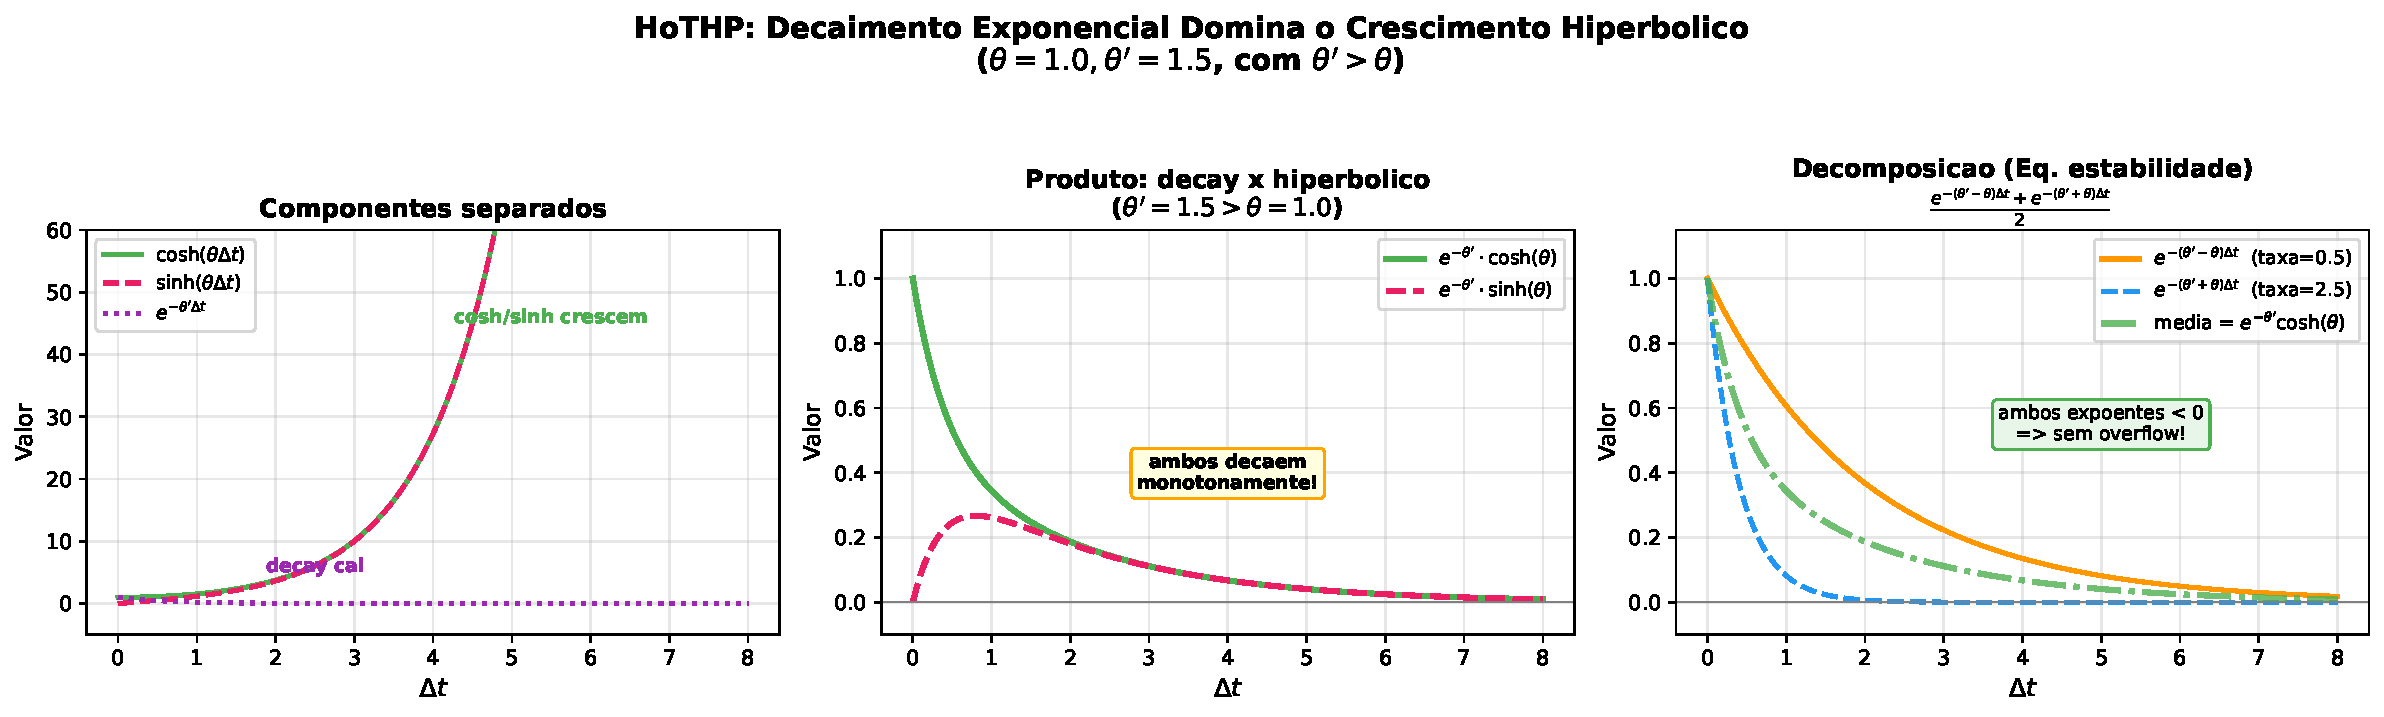
\includegraphics[width=\textwidth]{fig_decay_hiperbolico}
    \end{column}
  \end{columns}
\end{frame}

% Slide 24a: the score, one pair at a time
\begin{frame}{HoTHP score: one dimension-pair at a time}
  Each head splits into $d/2$ \textbf{pairs}. Pair $p$ has frequency $\theta_p$
  and components $(q_1^{(p)}, q_2^{(p)})$ and $(k_1^{(p)}, k_2^{(p)})$.
  \vspace{0.3em}
  \begin{block}{Score of one pair $=$ hyperbolic rotation by $\Delta t$}
    \[
      s^{(p)} = (q_1 k_1 + q_2 k_2)\,\cosh(\theta_p \Delta t)
              + (q_1 k_2 + q_2 k_1)\,\sinh(\theta_p \Delta t)
    \]
  \end{block}
  Full score $=$ sum over pairs, with the recency envelope $e^{-|\Delta t|\theta'}$
  and the usual $1/\sqrt{d}$ scaling ($\Delta t = t_i - t_j$):
  \[
    s_{ij} = \frac{1}{\sqrt{d}} \sum_{p=1}^{d/2}
      e^{-|\Delta t|\theta'}\; s^{(p)} .
  \]

\end{frame}

% Slide 24b: from cosh/sinh definitions down to the stable form
\begin{frame}{We never evaluate $\cosh/\sinh$, only exponentials}
  \textbf{Step 1.} Replace each by its definition ($\cosh$ is even, so
  $\theta_p\Delta t \to \theta_p|\Delta t|$):
  \[
    \cosh(\theta_p \Delta t) = \tfrac{1}{2}\big(e^{\theta_p|\Delta t|} + e^{-\theta_p|\Delta t|}\big),
    \qquad
    \sinh(\theta_p \Delta t) = \tfrac{\mathrm{sign}(\Delta t)}{2}\big(e^{\theta_p|\Delta t|} - e^{-\theta_p|\Delta t|}\big).
  \]
  \textbf{Step 2.} Multiply the $\cosh$ term by the envelope and \emph{merge the
  exponents} (this is the whole trick):
  \begin{align*}
    e^{-|\Delta t|\theta'}\cosh(\theta_p \Delta t)
      &= \tfrac{1}{2}\Big(
          e^{-|\Delta t|\theta'}\, e^{+\theta_p|\Delta t|}
        + e^{-|\Delta t|\theta'}\, e^{-\theta_p|\Delta t|}\Big) \\[0.3em]
      &= \tfrac{1}{2}\Big(
          e^{-|\Delta t|(\theta' - \theta_p)}
        + e^{-|\Delta t|(\theta' + \theta_p)}\Big).
  \end{align*}
  \textbf{Step 3.} Since $\theta' > \max_p \theta_p$ by construction, both
  $\theta'-\theta_p>0$ and $\theta'+\theta_p>0$: \alert{every exponent is
  negative}, so each term lands in $(0,1]$, no overflow, no \texttt{NaN}.
  \vspace{0.2em}
  {\small (The $\sinh$ term merges the same way, giving
  $\tfrac{\mathrm{sign}(\Delta t)}{2}\big(e^{-|\Delta t|(\theta'-\theta_p)} - e^{-|\Delta t|(\theta'+\theta_p)}\big)$.)}
\end{frame}

% Slide 25: architecture + where the bias acts
\begin{frame}{Architecture: where the exponential bias acts}
  HoTHP is a Transformer encoder with hyperbolic multi-head attention. \textbf{No}
  time information is added to the embedding; time enters only through the kernel.
  The bias acts in \textbf{two distinct steps}:
  \vspace{0.3em}
  \begin{enumerate}
    \item \textbf{Hyperbolic attention} $\to \mathbf{h}(t_j)$: the decay decides
          \emph{which past events} shape the hidden state. Recent events get more
          weight.
    \item \textbf{Intensity} $\lambda_k(t) = \mathrm{softplus}\!\big(
          \alpha_k (t-t_j) + \mathbf{w}_k^\top \mathbf{h}(t_j) + b_k\big)$:
          linear in the \emph{elapsed} time $t-t_j$, so shifting all timestamps
          changes nothing; $\alpha_k$ is free (can rise or fall after an event).
  \end{enumerate}
  \begin{block}{Consequence}
    The recency bias does \textbf{not} require the process to be self-exciting. It
    only requires that recent events be more informative. It helps on
    self-exciting \emph{and} self-inhibiting processes.
  \end{block}
\end{frame}

% Slide 26: kernel comparison zones
\begin{frame}{RoTHP vs. HoTHP kernel: training and extrapolation zones}
  \begin{figure}
    \centering
    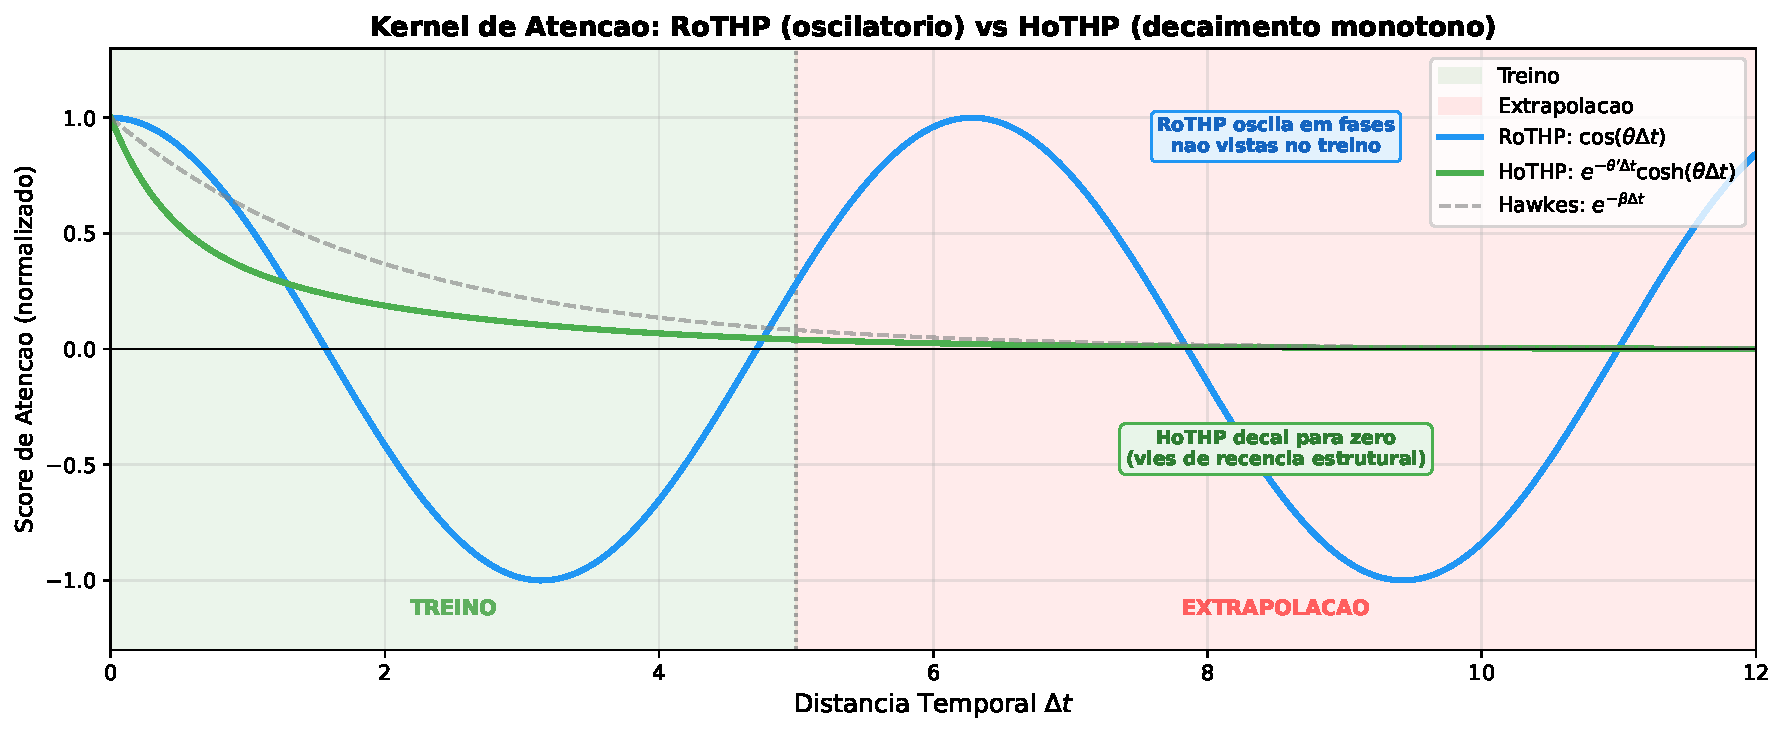
\includegraphics[width=0.74\textwidth]{fig_kernel_rothp_vs_hothp}
  \end{figure}
  \vspace{-0.3em}
  {\small In the \textbf{training zone}, both models fit the data. In the
  \textbf{extrapolation zone}, the RoTHP trigonometric kernel keeps oscillating in
  unseen phases, while the HoTHP hyperbolic kernel decays exponentially to zero,
  without oscillation, like the classical Hawkes kernel (dashed).}
\end{frame}

% ============================================================
\section{Experiments and results}
% ============================================================

% Slide 27: setup
\begin{frame}{Experimental setup}
  \begin{itemize}
    \item \textbf{Synthetic data:} multivariate Hawkes with exponential kernel,
          two regimes: \emph{slow decay} ($\beta$ small) and \emph{fast decay}
          ($\beta$ large). We know the ground truth.
    \item \textbf{Real data (EasyTPP \cite{xue2024easytpp}):} Taxi, StackOverflow,
          Amazon, Retweet.
    \item \textbf{Protocol:} train short, test long, factors
          $\alpha \in \{1,2,5,10\}$ (synthetic) and $\{1,2,5\}$ (real).
    \item \textbf{Models:} NHP, THP, RoTHP, HoTHP. THP/RoTHP/HoTHP share the same
          architecture and intensity, differing \textbf{only in how time enters
          the attention} (a controlled comparison).
    \item \textbf{Metrics:} NLL (main), RMSE, type accuracy. Synthetic: 10 seeds +
          Wilcoxon signed-rank test. Real: 3 seeds (no Wilcoxon).
  \end{itemize}
\end{frame}

% Slide 28: synthetic NLL table
\begin{frame}{Synthetic results: NLL under extrapolation}
  \begin{table}
    \centering \small
    \begin{tabular}{llcccc}
      \toprule
      Scenario & Model & $1\times$ & $2\times$ & $5\times$ & $10\times$ \\
      \midrule
      \multirow{4}{*}{Slow decay}
        & NHP    & $\mathbf{1.470}$ & $2.197$ & $2.667$ & $\underline{2.817}$ \\
        & THP    & $\underline{1.475}$ & $3.926$ & $4.127$ & $4.199$ \\
        & RoTHP  & $1.499$ & $\underline{2.007}$ & $\underline{2.642}$ & $3.001$ \\
        & HoTHP  & $1.545$ & $\mathbf{1.609}$ & $\mathbf{1.943}$ & $\mathbf{2.364}$ \\
      \midrule
      \multirow{4}{*}{Fast decay}
        & NHP    & $\mathbf{1.663}$ & $\underline{1.833}$ & $\underline{2.057}$ & $\underline{2.153}$ \\
        & THP    & $\underline{1.677}$ & $3.391$ & $3.761$ & $3.897$ \\
        & RoTHP  & $1.681$ & $2.039$ & $2.146$ & $2.275$ \\
        & HoTHP  & $1.689$ & $\mathbf{1.701}$ & $\mathbf{1.740}$ & $\mathbf{1.774}$ \\
      \bottomrule
    \end{tabular}
  \end{table}
  \vspace{0.2em}
  {\small NLL (mean, 10 seeds), lower is better. \textbf{HoTHP wins at every
  extrapolation factor} ($2\times, 5\times, 10\times$) in both scenarios; the small
  cost at $1\times$ reverses immediately. Advantage significant (Wilcoxon,
  $p<0.05$) in all cases.}
\end{frame}

% Slide 29: synthetic NLL figure
\begin{frame}{Synthetic results: NLL vs. extrapolation factor}
  \begin{figure}
    \centering
    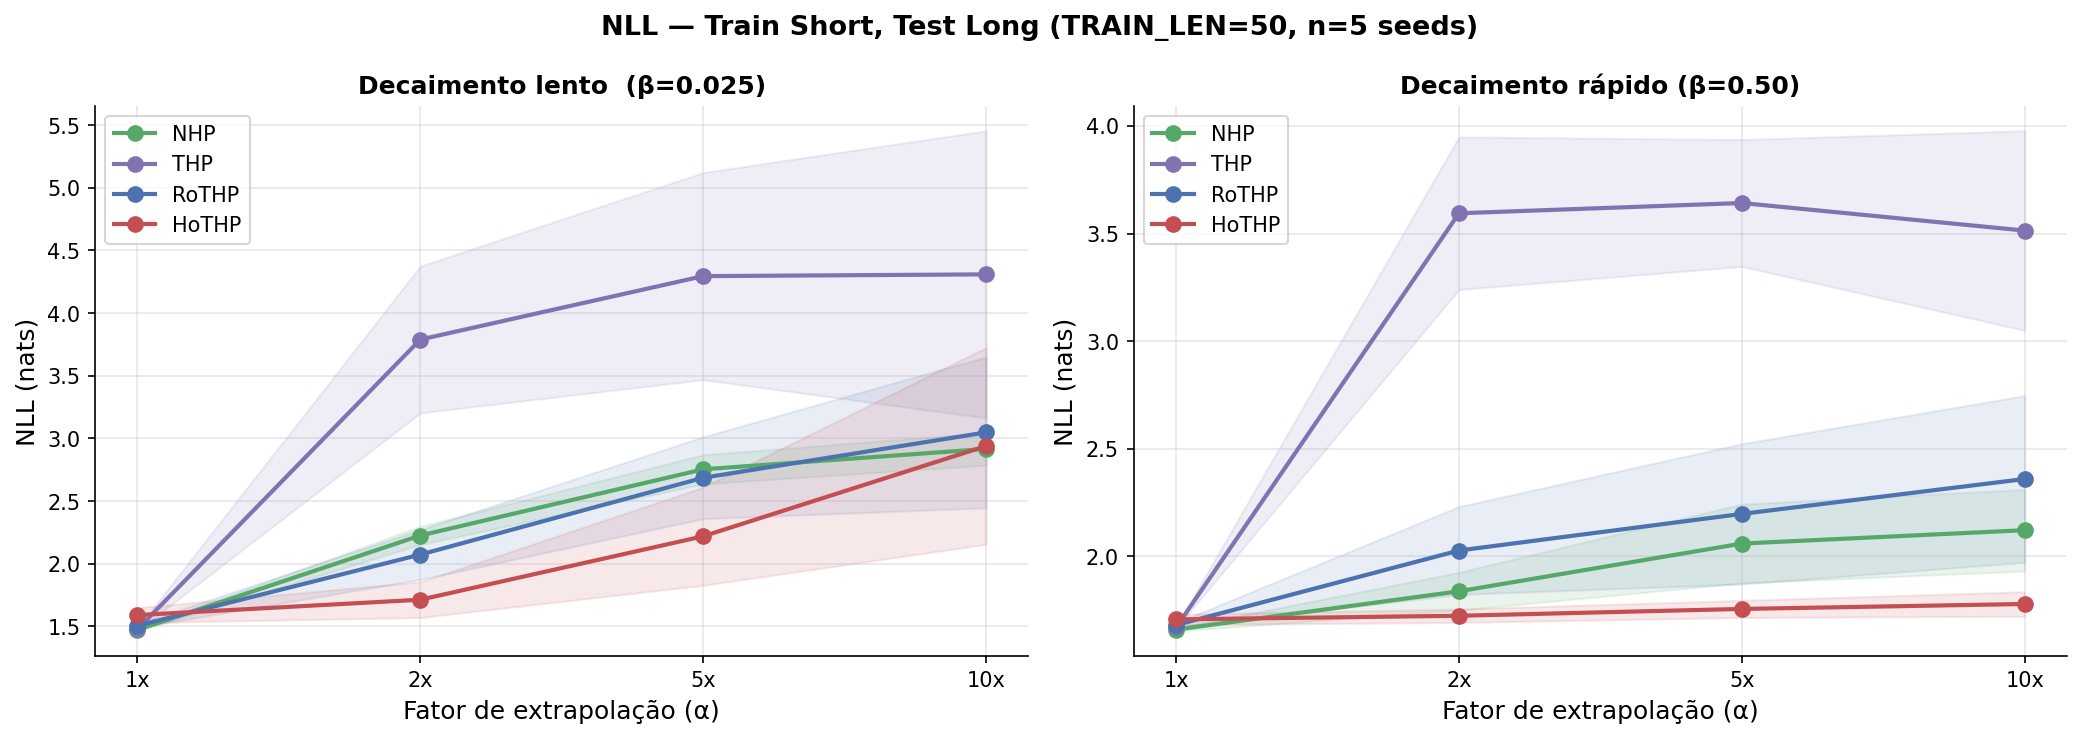
\includegraphics[width=0.9\textwidth]{fig_extrapolation_nll_sintetico}
  \end{figure}
  \vspace{-0.3em}
  {\small In fast decay, the HoTHP NLL grows only $0.085$ from $1\times$ to
  $10\times$ (almost flat), while the THP diverges and RoTHP/NHP degrade more. The
  recency bias is aligned with the exponential kernel that generated the data.}
\end{frame}

% Slide 30: synthetic RMSE
\begin{frame}{Synthetic results: RMSE}
  \begin{figure}
    \centering
    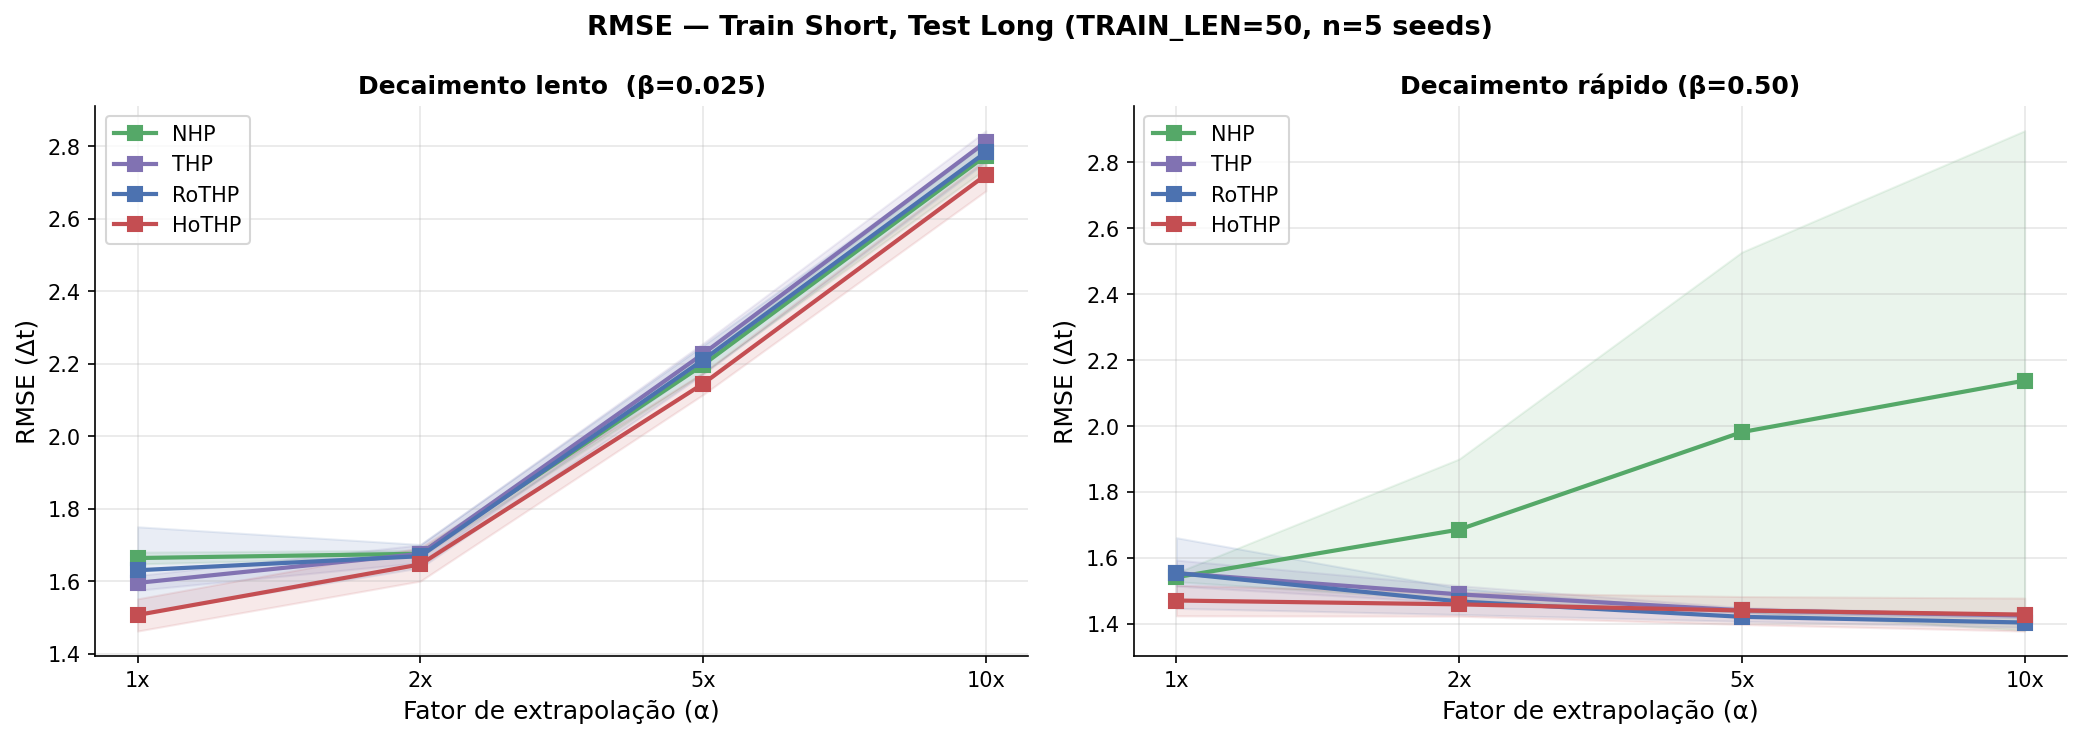
\includegraphics[width=0.9\textwidth]{fig_extrapolation_rmse_sintetico}
  \end{figure}
  \vspace{-0.3em}
  {\small Unlike the NLL, the RMSE does not separate the models: they stay close
  at every factor. The HoTHP advantage shows up in the \textbf{likelihood}
  (modeling the full temporal distribution), not in the pointwise prediction of
  the next interval.}
\end{frame}

% Slide 31: real datasets + NLL table
\begin{frame}{Real data: datasets and NLL}
  \begin{columns}[T]
    \begin{column}{0.36\textwidth}
      {\scriptsize
      \begin{tabular}{lcc}
        \toprule
        Dataset & Types & $L_{\text{train}}$ \\
        \midrule
        Amazon        & 16 & 18 \\
        StackOverflow & 22 & 20 \\
        Taxi          & 10 & 7  \\
        Retweet       & 3  & 50 \\
        \bottomrule
      \end{tabular}}
      \vspace{0.6em}

      {\scriptsize Raw timestamps (shift to zero only), 3 seeds. Retweet is
      studied separately (ablation).}
    \end{column}
    \begin{column}{0.62\textwidth}
      {\scriptsize
      \begin{tabular}{llccc}
        \toprule
        Dataset & Model & $1\times$ & $2\times$ & $5\times$ \\
        \midrule
        \multirow{4}{*}{Taxi}
          & THP   & $-0.273$ & $-0.314$ & $-0.243$ \\
          & RoTHP & $-0.271$ & $-0.317$ & $-0.137$ \\
          & HoTHP & $\underline{-0.278}$ & $\underline{-0.328}$ & $\underline{-0.266}$ \\
          & NHP   & $\mathbf{-0.449}$ & $\mathbf{-0.506}$ & $\mathbf{-0.460}$ \\
        \midrule
        \multirow{4}{*}{Amazon}
          & THP   & $2.264$ & $2.237$ & $2.254$ \\
          & RoTHP & $2.268$ & $2.230$ & $2.247$ \\
          & HoTHP & $\underline{2.263}$ & $\underline{2.207}$ & $\underline{2.187}$ \\
          & NHP   & $\mathbf{0.658}$ & $\mathbf{0.630}$ & $\mathbf{0.638}$ \\
        \midrule
        \multirow{4}{*}{StackOv.}
          & THP   & $\underline{2.744}$ & $\underline{2.642}$ & $\mathbf{2.519}$ \\
          & RoTHP & $2.766$ & $2.655$ & $2.545$ \\
          & HoTHP & $2.758$ & $2.649$ & $2.536$ \\
          & NHP   & $\mathbf{2.742}$ & $\mathbf{2.633}$ & $\underline{2.524}$ \\
        \bottomrule
      \end{tabular}}
    \end{column}
  \end{columns}
  \vspace{0.3em}
  {\small Within the Transformer family, HoTHP has the best NLL on Amazon and Taxi
  at every factor, and is the only one that keeps \emph{improving} on Amazon as the
  sequence grows.}
\end{frame}

% Slide 32: accuracy - HoTHP leads on the datasets where recency helps
\begin{frame}{Real data: type-prediction accuracy}
  \begin{columns}[T]
    \begin{column}{0.5\textwidth}
      {\scriptsize
      \begin{tabular}{llccc}
        \toprule
        Dataset & Model & $1\times$ & $2\times$ & $5\times$ \\
        \midrule
        \multirow{4}{*}{Amazon}
          & NHP   & $.293$ & $.306$ & $.315$ \\
          & THP   & $.308$ & $.317$ & $.314$ \\
          & RoTHP & $.308$ & $.323$ & $.320$ \\
          & HoTHP & $\mathbf{.312}$ & $\mathbf{.331}$ & $\mathbf{.340}$ \\
        \midrule
        \multirow{4}{*}{StackOv.}
          & NHP   & $.469$ & $.462$ & $.445$ \\
          & THP   & $.473$ & $.466$ & $.450$ \\
          & RoTHP & $.473$ & $.464$ & $.448$ \\
          & HoTHP & $\mathbf{.474}$ & $\mathbf{.466}$ & $\mathbf{.451}$ \\
        \midrule
        \multirow{4}{*}{Retweet\textsuperscript{$\dagger$}}
          & NHP   & --- & --- & --- \\
          & THP   & $.590$ & $.596$ & $.597$ \\
          & RoTHP & $.590$ & $.594$ & $.589$ \\
          & HoTHP & $\mathbf{.595}$ & $\mathbf{.601}$ & $\mathbf{.600}$ \\
        \bottomrule
      \end{tabular}}
    \end{column}
    \begin{column}{0.48\textwidth}
      \centering
      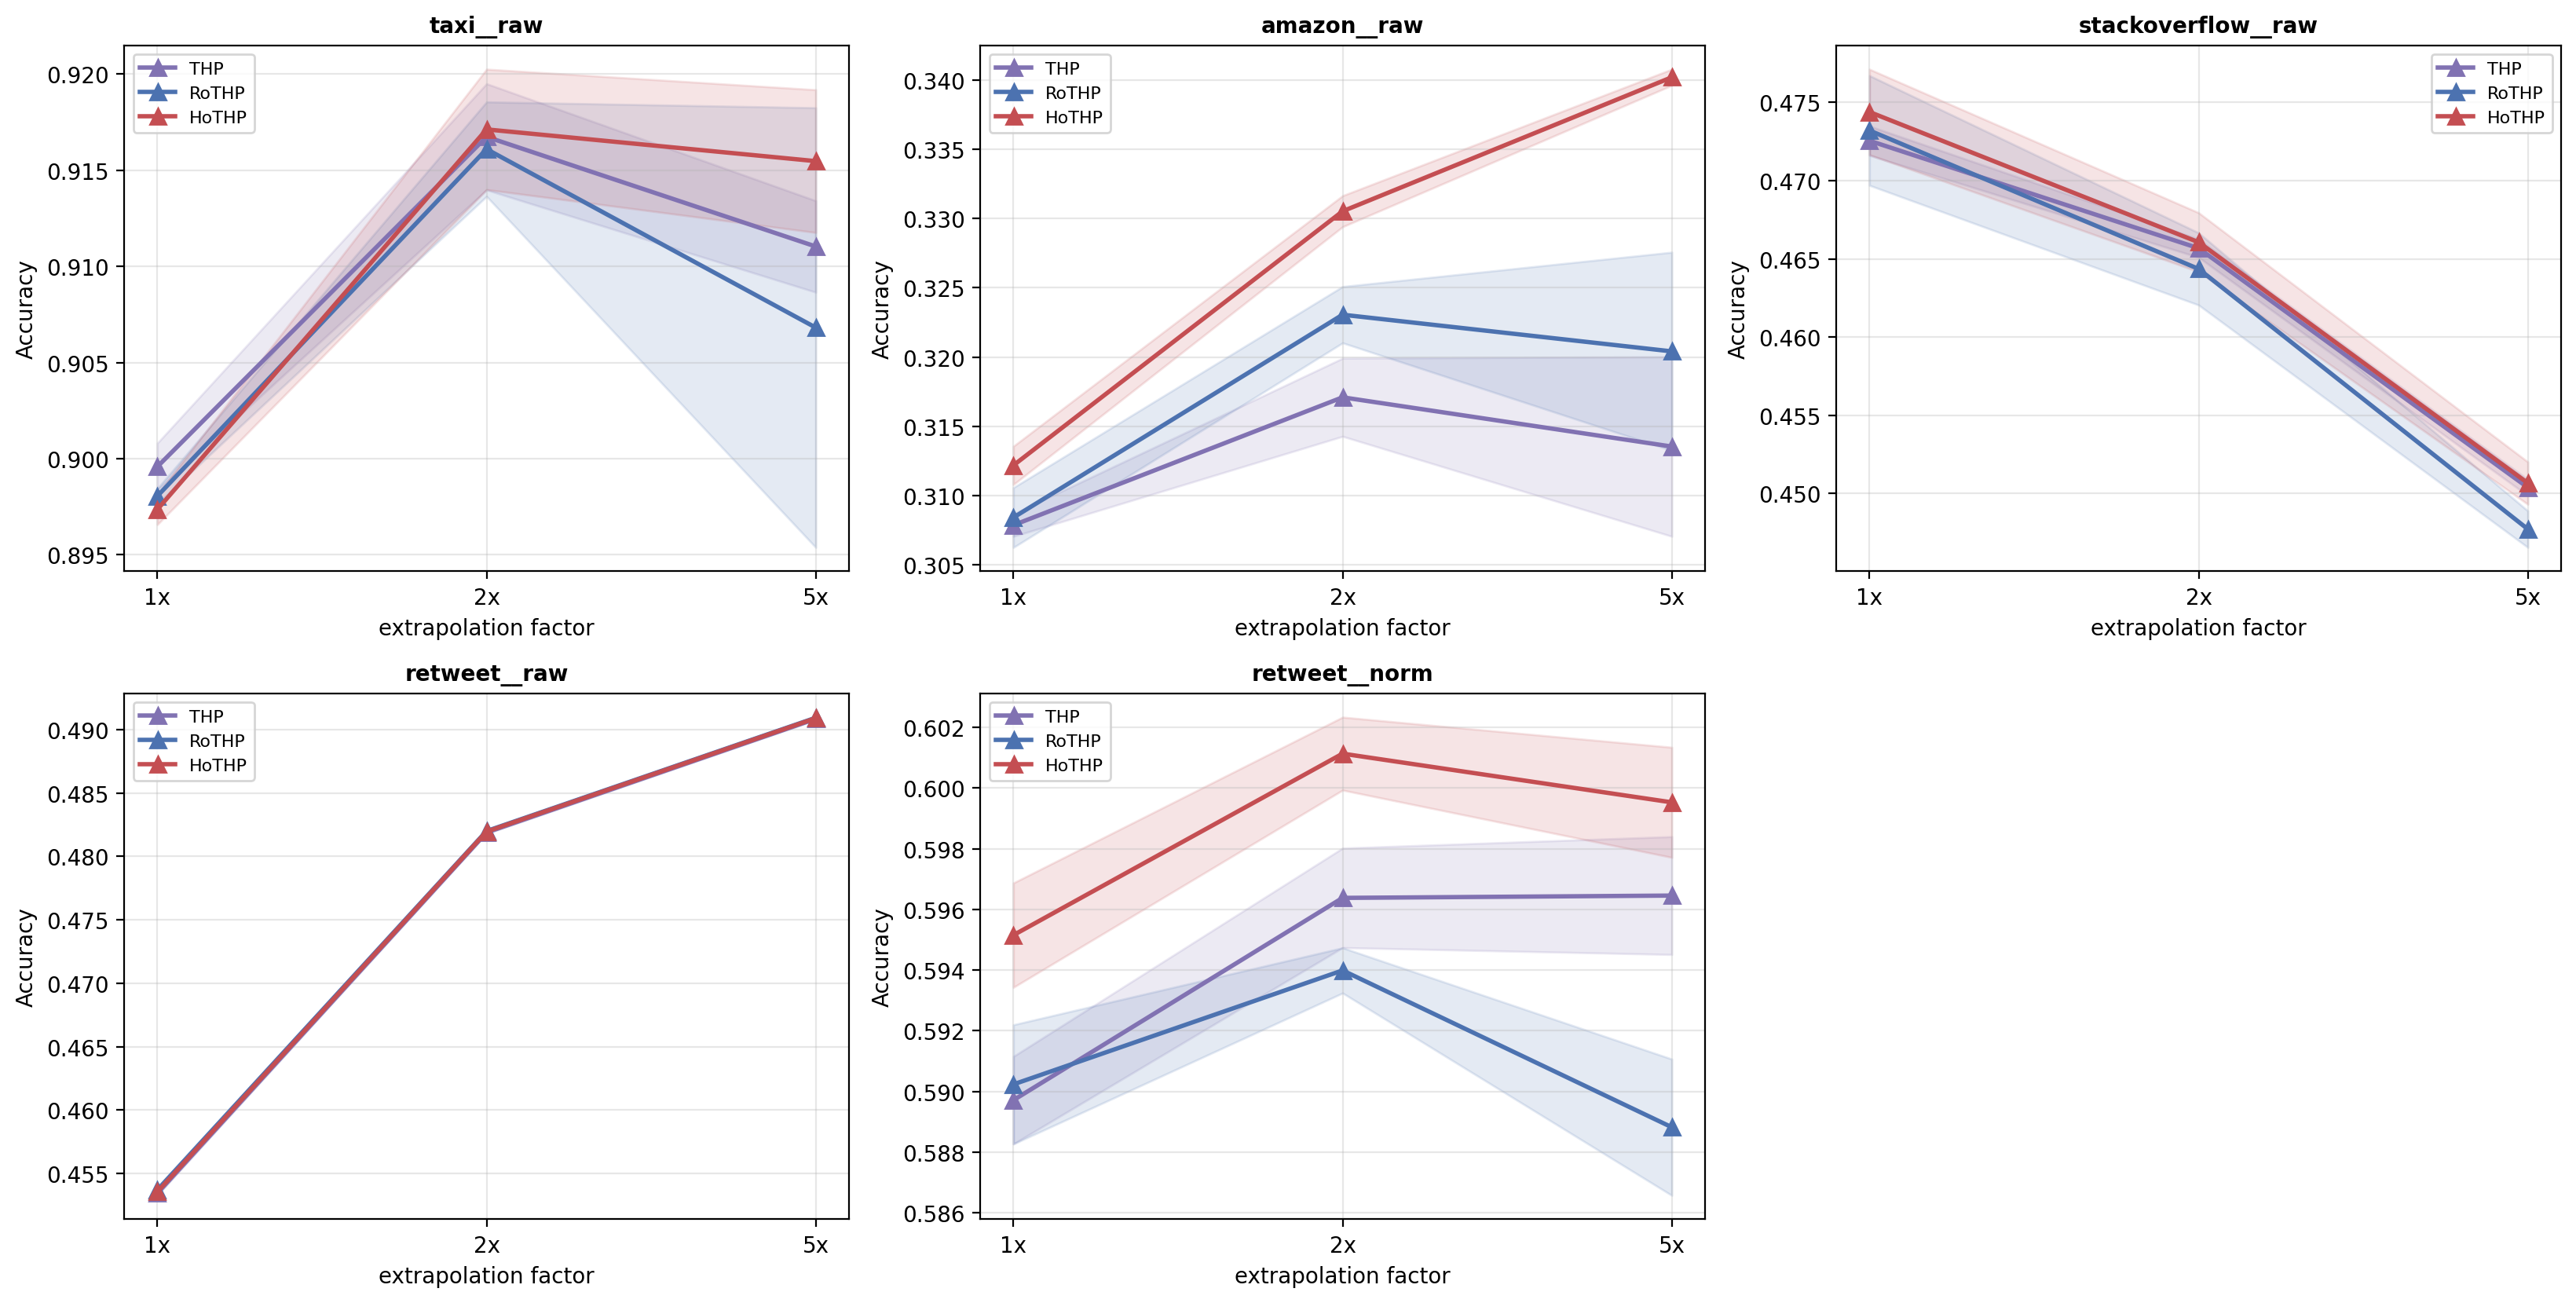
\includegraphics[width=\textwidth]{fig_real_acc}

      \vspace{0.4em}
      {\scriptsize $\dagger$ Retweet normalized (raw timestamps overflow all
      Transformers); NHP not run there.}
    \end{column}
  \end{columns}
  \vspace{0.1em}
  {\small HoTHP has the \textbf{best accuracy at every factor, on every dataset
  where recency helps}. It beats the Transformer family and also NHP, whose lead
  was confined to NLL. On Amazon the margin \emph{grows} with the sequence length
  ($+0.020$ over the best baseline at $5\times$).}
\end{frame}

% Slide 33: learned intensities
\begin{frame}{What the models learn: conditional intensities}
  \begin{columns}[T]
    \begin{column}{0.46\textwidth}
      \centering
      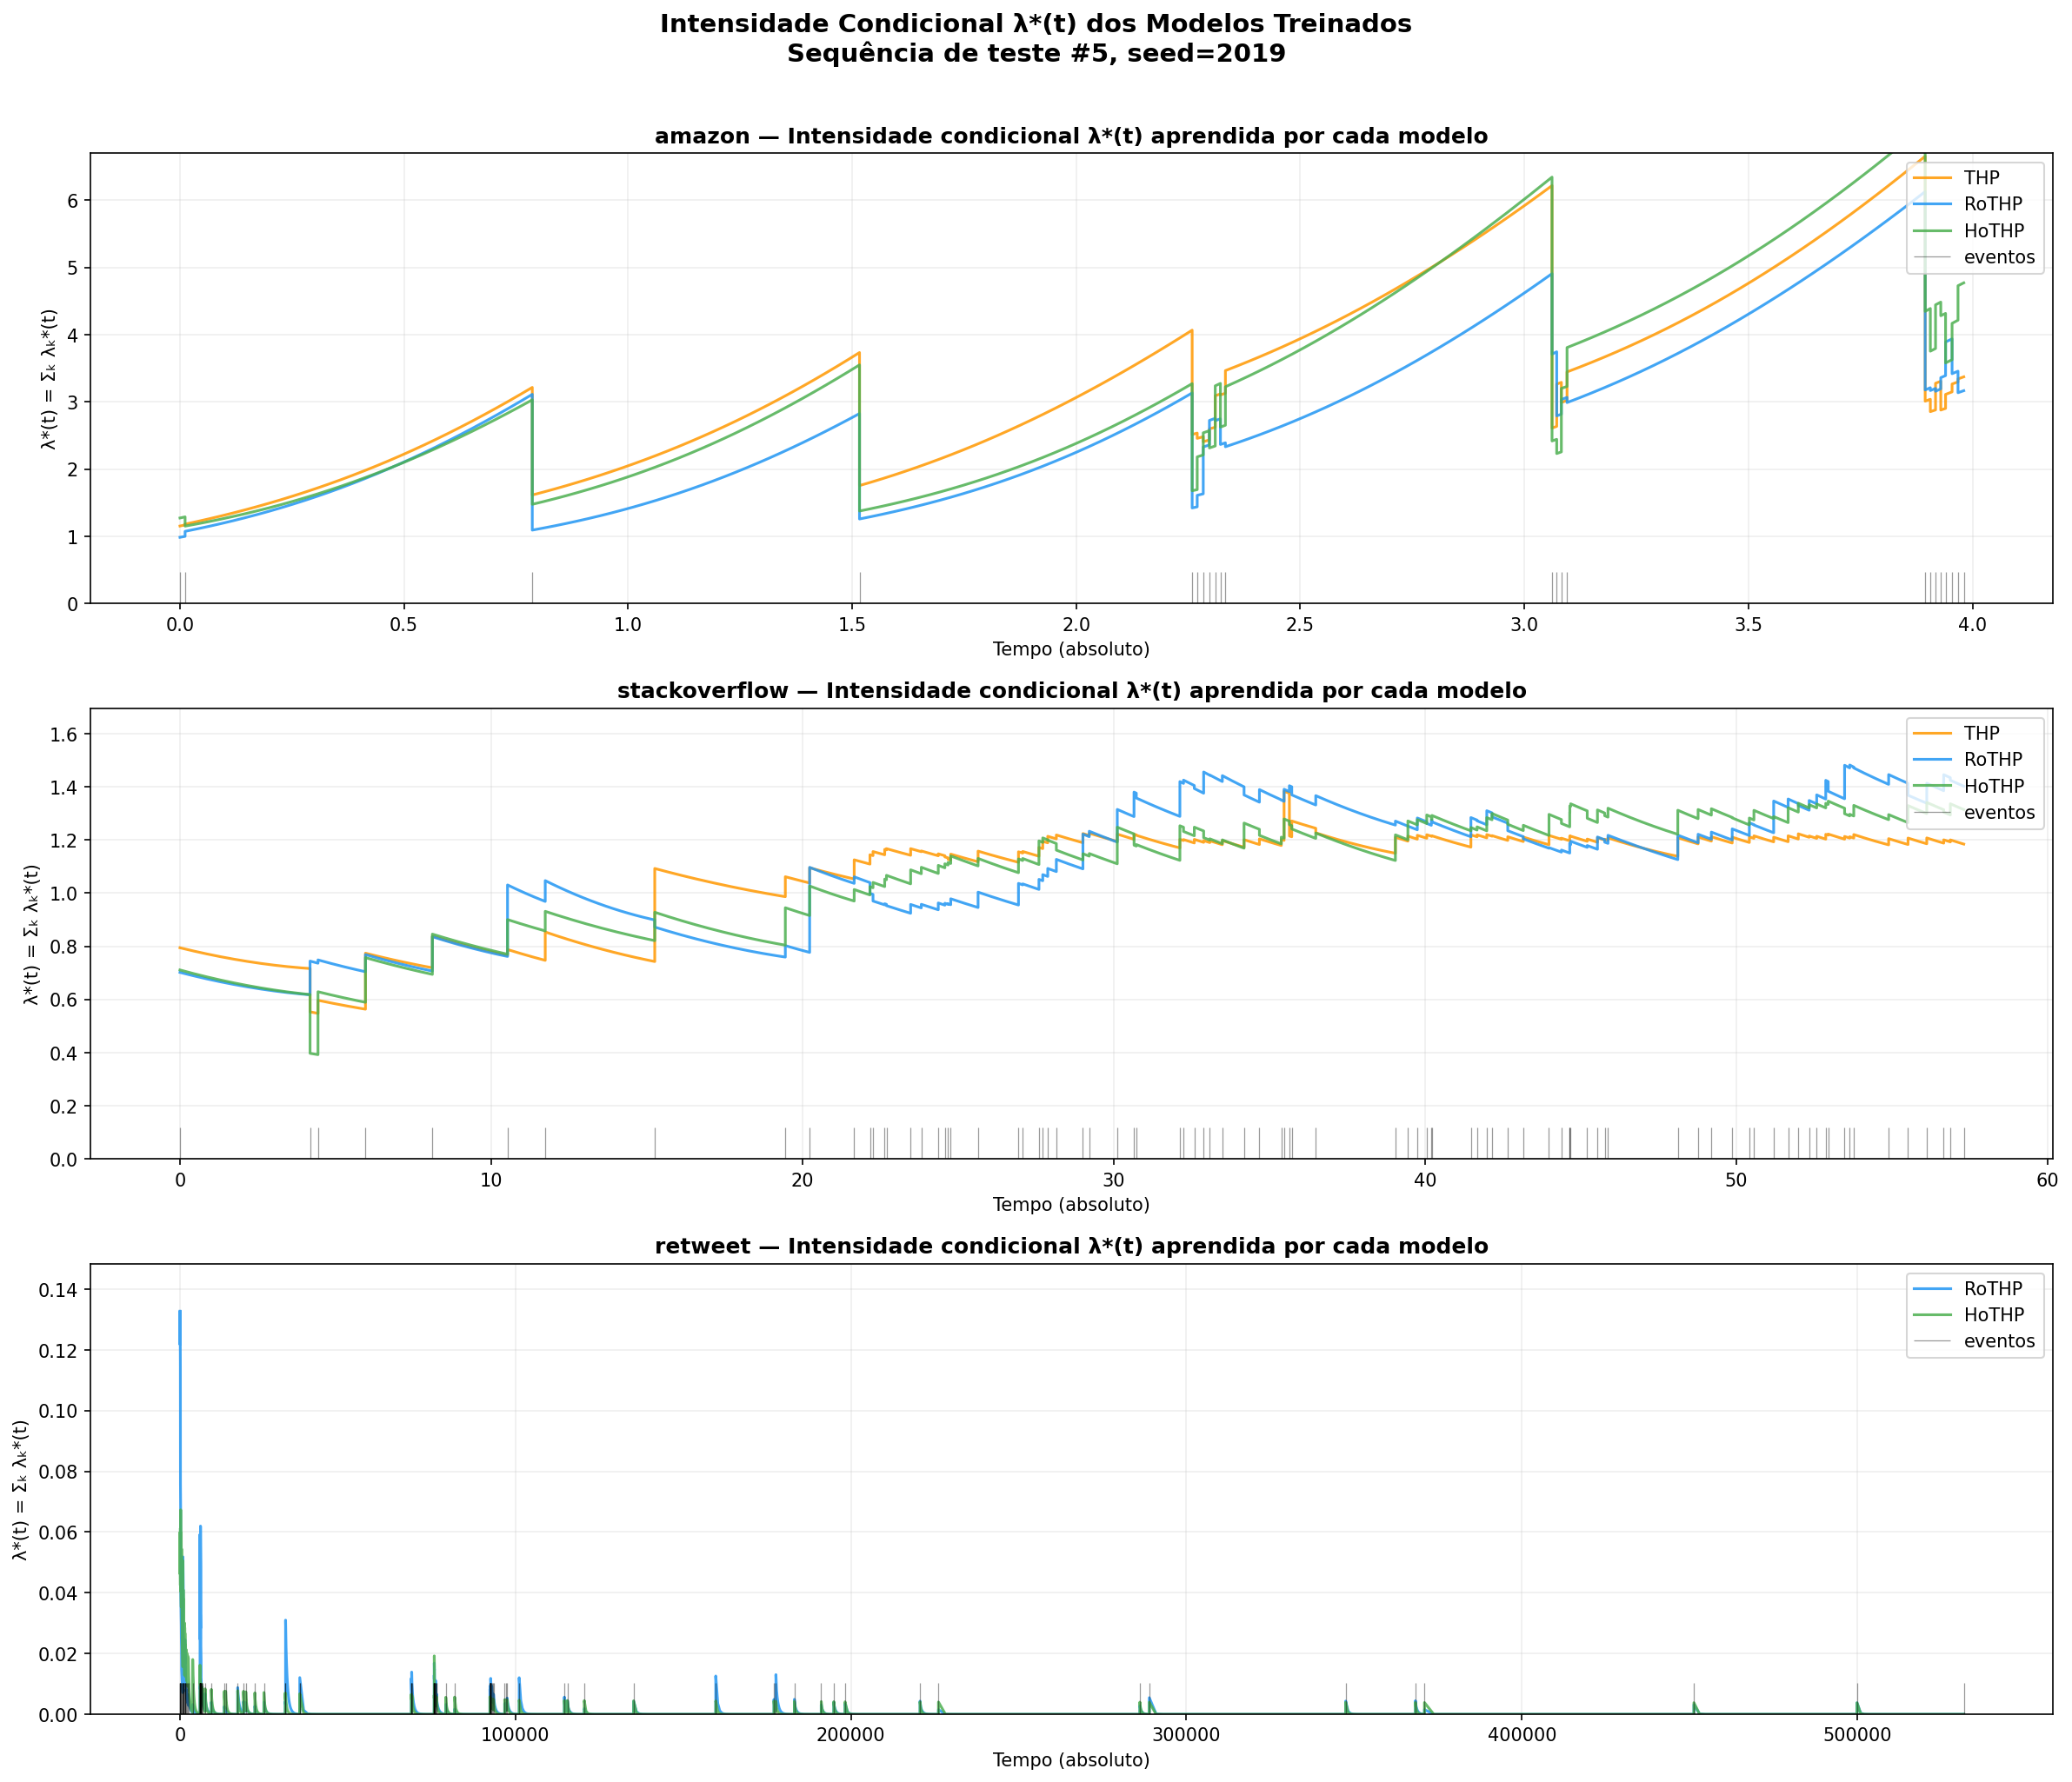
\includegraphics[height=0.66\textheight]{fig_model_intensity}
    \end{column}
    \begin{column}{0.52\textwidth}
      \small
      Learned $\lambda^*(t)$ on representative test sequences:
      \begin{itemize}
        \small
        \item \textbf{Amazon:} intensity grows between events and falls at each
              event (\emph{self-inhibiting}). Yet HoTHP wins: the most recent
              event is still the most informative.
        \item \textbf{StackOverflow:} intensity is almost flat (little temporal
              memory); the models tie.
        \item \textbf{Retweet:} models react only to the initial burst, then
              collapse to $\lambda^* \approx 0$ (extreme temporal scale).
      \end{itemize}
      \vspace{-0.3em}
      \begin{block}{Confirms the two-step view}
        \small The recency bias acts on \textbf{attention} (which past events
        matter), not on the intensity sign. That is why it helps even on a
        self-inhibiting process.
      \end{block}
    \end{column}
  \end{columns}
\end{frame}

% Slide 34: Retweet ablation + cost
\begin{frame}{Ablation on Retweet, and computational cost}
  \begin{columns}[T]
    \begin{column}{0.5\textwidth}
      \textbf{Retweet: scale or bias?}
      {\scriptsize
      \begin{tabular}{llcc}
        \toprule
        Version & Model & $1\times$ & $5\times$ \\
        \midrule
        \multirow{3}{*}{Raw}
          & THP   & $15.9$ & $2.3{\times}10^{4}$ \\
          & RoTHP & $15.9$ & $7.0{\times}10^{5}$ \\
          & HoTHP & $15.9$ & $1.4{\times}10^{5}$ \\
        \midrule
        \multirow{3}{*}{Norm.}
          & THP   & $\mathbf{-2.180}$ & $\underline{0.039}$ \\
          & RoTHP & $-2.133$ & $47.6$ \\
          & HoTHP & $\underline{-2.139}$ & $\mathbf{-0.651}$ \\
        \bottomrule
      \end{tabular}}
      \vspace{0.4em}

      {\small The problem was the \textbf{scale}. After normalization, HoTHP is the
      only model with a negative (stable) NLL at $5\times$.}
    \end{column}
    \begin{column}{0.5\textwidth}
      \textbf{Cost vs. benefit}
      \begin{itemize}
        \small
        \item HoTHP computes the kernel per event \emph{pair}: $O(L^2)$.
        \item On real data it is $1.07\times$ (Taxi) to $2.44\times$ (Retweet)
              slower than RoTHP, but \textbf{cheaper than the NHP} (the strongest
              NLL baseline).
        \item Cost is paid once, at training. At inference, what matters is a
              \emph{valid} result: RoTHP at $5\times$ gives NLL $47.6$, HoTHP gives
              $-0.651$.
      \end{itemize}
    \end{column}
  \end{columns}
\end{frame}

% ============================================================
\section{Conclusion}
% ============================================================

% Slide: what changed since the qualification (committee feedback)
\begin{frame}{Since the qualification}
  Following the committee's feedback (qualification, 10 July 2026), the
  dissertation was revised on four fronts:
  \vspace{0.4em}
  \begin{itemize}
    \item \textbf{Notation and readability:} acronyms expanded in the abstract, a
          list of symbols added, unified notation ($\gamma_k$ for the intensity
          slope, $\rho$ for the extrapolation factor), and the modulus corrected
          in the kernel equation ($e^{-|\Delta t|\theta'}$).
    \item \textbf{Deeper foundations:} a Poisson--Hawkes taxonomy, the explicit
          Poisson\,$\to$\,Hawkes likelihood link, and a discussion of the RoPE
          period limitation.
    \item \textbf{More results:} RMSE now reported on the real datasets, and
          sources added to every reused figure.
    \item \textbf{Writing:} the conclusion and the future-work chapter completed.
  \end{itemize}
\end{frame}

% Slide 35: contributions
\begin{frame}{Contributions}
  \begin{itemize}
    \item \textbf{HoTHP:} a Transformer Hawkes Process with a \textbf{hyperbolic}
          rotary kernel, combining time-invariance with a structural exponential
          recency bias in a single attention mechanism.
    \item A learnable $\theta'$, parametrized so that $\theta' > \max_j \theta_j$
          \textbf{by construction}, guaranteeing exponential decay of the score
          and numerical stability.
    \item Under \emph{train short, test long}, HoTHP keeps the NLL stable up to
          $10\times$ on synthetic data (significant by Wilcoxon), and is the best
          of the Transformer family on Amazon and Taxi.
    \item An analysis separating \emph{where} the bias acts (attention vs.
          intensity), explaining why it helps even on self-inhibiting processes.
    \item Implementation and experiments in the EasyTPP framework.
  \end{itemize}
\end{frame}

% Slide: limitations and future work
\begin{frame}{Limitations and future work}
  \textbf{Limitations}
  \begin{itemize}
    \item The exponential bias hurts when distant events are as relevant as recent
          ones (long-range memory).
    \item Extreme temporal scales need normalization to avoid numerical saturation
          (as on raw Retweet).
    \item $\theta'$ is a \textbf{single global} decay rate; processes with multiple
          temporal scales may require multiple rates.
  \end{itemize}
  \vspace{0.2em}
  \textbf{Future work}
  \begin{itemize}
    \item \textbf{Multiple decay scales:} one learnable $\theta'$ per head
          (ALiBi-style), each specializing in a temporal scale.
    \item \textbf{Alternative decay shapes:} power-law instead of exponential,
          for long-range memory (aftershocks, cascades).
    \item \textbf{Broader evaluation:} long-horizon benchmarks (HoTPP), new domains.
    \item \textbf{Beyond attention:} does the recency bias transfer to state-space
          models (Mamba) and LLM-based TPPs?
  \end{itemize}
\end{frame}

% Slide 38: thanks
\begin{frame}{Thank you}
  \begin{center}
    \large \textbf{Hugo Ramos Soares} \\
    \normalsize
    Universidade Federal do Ceará \\
    Orientador: César Lincoln C. Mattos \\
    Coorientador: João Paulo Pordeus Gomes \\
  \end{center}
\end{frame}

% References (real frame so BibTeX runs and \cite{} resolves)
\begin{frame}[noframenumbering,allowframebreaks]{References}
  \setbeamertemplate{bibliography item}{\insertbiblabel}
  \scriptsize
  \bibliographystyle{plain}
  \bibliography{refs}
\end{frame}

% ============================================================
% BACKUP SLIDES (not counted, shown only if the committee asks)
% ============================================================
\appendix

% Backup D2: the most important expected question
\begin{frame}[noframenumbering]{Backup: why hyperbolic, not a single $e^{-\beta|\Delta t|}$ or ALiBi?}
  Expanding the score gives a \textbf{content-weighted mixture of exponentials}:
  \[
    s_{ij} = \frac{1}{\sqrt d}\sum_{p=1}^{d/2}\Big[
      c_p(\mathbf{q},\mathbf{k})\,e^{-(\theta'-\theta_p)|\Delta t|}
    + d_p(\mathbf{q},\mathbf{k})\,e^{-(\theta'+\theta_p)|\Delta t|}\Big]
  \]
  Three things a single $e^{-\beta|\Delta t|}$ or an ALiBi bias do \textbf{not} give:
  \begin{enumerate}
    \item \textbf{Content-dependent coefficients} $c_p, d_p$ (the $\mathbf{q}\cdot\mathbf{k}$
          products per dimension pair), which can be positive or negative; ALiBi's
          penalty is fixed and content-independent.
    \item \textbf{A spectrum of decay rates} $\{\theta'-\theta_p,\ \theta'+\theta_p\}$:
          since $\theta_p$ ranges from $1$ down to $\sim 10^{-4}$, slow components
          ($\theta'-\theta_1$, near zero) keep longer memory while fast components
          ($\theta'+\theta_p$) forget quickly. A single $\beta$ has one scale.
    \item \textbf{Time-invariance} (the score depends only on $\Delta t$), which the
          discrete ALiBi does not provide in continuous time.
  \end{enumerate}
\end{frame}

% Backup D8: is the Transformer family competitive? + THP replication finding
\begin{frame}[noframenumbering]{Backup: is the Transformer family competitive? (NHP vs THP)}
  \textbf{NHP wins NLL on Amazon/Taxi: expected, not a bug.} It matches the
  EasyTPP benchmark: continuous-time recurrent models fit the inter-event density
  natively. Our question is \emph{within-family} (fixed architecture, only the
  kernel changes): HoTHP is the best of the three, beats NHP on \textbf{accuracy}
  (Amazon, SO), and beats \emph{all} baselines on synthetic NLL (10 seeds, Wilcoxon).
  \vspace{0.3em}
  \begin{block}{We also investigated the NHP\,$>$\,THP inversion directly}
    Reproducing the \textbf{original} THP on its own MIMIC-II data:
    \begin{itemize}
      \item Under a consistent integration routine, NHP $\geq$ THP even there.
      \item The THP paper's high log-likelihood is an artifact of its Monte-Carlo
            solver variant: the \textbf{implementation} effect on LL ($\approx 2.76$
            nats) is about $10\times$ the \textbf{model} effect ($\approx 0.28$ nats).
    \end{itemize}
    So log-likelihoods from different implementations are not directly comparable.
    The inversion is not an artifact of our reimplementation.
  \end{block}
  {\footnotesize (Complementary investigation, in a separate codebase; not a chapter of the dissertation.)}
\end{frame}

% Backup J2: learned theta' values -- PLACEHOLDER, fill before the defense
\begin{frame}[noframenumbering]{Backup: what did $\theta'$ converge to?}
  Parametrized so that $\theta' = \mathrm{softplus}(\text{raw}) + 1 + 10^{-4}
  > \max_p \theta_p = 1$ \textbf{by construction}.
  \vspace{0.4em}
  \begin{center}
    \begin{tabular}{lc}
      \toprule
      Scenario / dataset & Learned $\theta'$ \\
      \midrule
      Synthetic, fast decay & \alert{[fill]} \\
      Synthetic, slow decay & \alert{[fill]} \\
      Amazon / Taxi / StackOverflow & \alert{[fill]} \\
      \bottomrule
    \end{tabular}
  \end{center}
  \vspace{0.4em}
  \textbf{Expectation:} in \emph{fast decay}, $\theta'$ larger (shorter memory);
  in \emph{slow decay}, $\theta'$ smaller.
  \vspace{0.3em}

  {\footnotesize \alert{TODO before the defense:} extract
  $\theta' = \mathrm{softplus}(\text{raw})+1+10^{-4}$ from the checkpoints and fill
  the table.}
\end{frame}

% Backup D6: the compensator integral (the "Monte Carlo" terminology point)
\begin{frame}[noframenumbering]{Backup: how is the compensator integral computed?}
  \begin{itemize}
    \item The \textbf{same routine} for all four models, defined once in the EasyTPP
          base class.
    \item A \textbf{deterministic grid} of 20 nodes per inter-event interval (a fixed
          \texttt{linspace} quadrature; the text calls it Monte Carlo).
    \item \textbf{Key point:} any estimator bias is \emph{identical} across models, so
          the NLL ranking does not depend on the integral approximation.
  \end{itemize}
\end{frame}

\end{document}
